\documentclass[11pt]{article}
\usepackage[margin=1in]{geometry}
\usepackage{booktabs}
\usepackage{array}
\usepackage{longtable}
\usepackage{amsmath}
\usepackage{graphicx}
\usepackage{caption}
\usepackage{float}
\usepackage[table]{xcolor}
\usepackage{tikz}
\usetikzlibrary{arrows.meta,positioning,backgrounds,fit}
\usepackage[hidelinks]{hyperref}
\definecolor{vgreen}{HTML}{1B7837}
\definecolor{vorange}{HTML}{C97A0A}
\definecolor{vred}{HTML}{C0392B}
\definecolor{vgray}{HTML}{555555}
\definecolor{fd1c}{HTML}{1f77b4}
\definecolor{fd3c}{HTML}{C0392B}
\newcommand{\ttt}[1]{\texttt{#1}}
\newcommand{\verd}[2]{\textcolor{#1}{\textbf{#2}}}
\setlength{\parindent}{0pt}
\setlength{\parskip}{0.55em}


\begin{document}

\title{\textbf{Connectomic identification and sensorimotor partners of the FD3 figure-detection cell (\ttt{LPT42\_Nod4})}}

\author{Stage 7 FD3 Identification}

\date{\today}

\maketitle

\tableofcontents

\part{Identity: FD3 is \texttt{LPT42\_Nod4}}

\textbf{Summary.}\quad Egelhaaf defined FD3 as a regressive, fronto-lateral figure-detection cell with a frontal gap, small-field preference, contralateral inhibition, and a heterolateral noduli-group projection. This report identifies the FlyWire cell type \textbf{\ttt{LPT42\_Nod4}} as the connectomic correlate of that FD3 phenotype. The candidate draws 98.58\% of its measured T4/T5 motion input from the back-to-front lobula-plate layer, has a receptive field shifted laterally relative to FD1 while leaving the FD1 frontal band nearly empty, pools a spatially bounded input patch, is cholinergic, and sends most output contralaterally (90.33\%). Among 5 nearby Nod/LPT candidate types, it is the strongest FD3 match and its own strongest FD-family match. The evidence is therefore a convergent anatomical identification, not a new physiology recording. The primary numbers in this report come from the \ttt{offline} track. The v630 cross-version check is not claimed here because it was unavailable in the present run (v630 cross-check is live-only); left/right agreement and offline reproducibility are reported explicitly.

\section{Introduction}

\textbf{Figure-ground discrimination and the FD cells.}\quad
A textured object is invisible against a matched background until it moves at a different
velocity or phase; relative motion then makes it salient. Reichardt and Poggio showed
behaviourally that flies detect and track such figures, and that the effect depends on relative
phase and on the figure being small relative to the background~\cite{rp1979}. Egelhaaf, in a three-part
study, asked which neurons could implement this~\cite{egelhaaf1985a,egelhaaf1985b,egelhaaf1985c}.
Part~II described a new class of
lobula-plate tangential cells, the \emph{figure-detection} (FD) cells, defined functionally by a
stronger response to a small moving figure than to wide-field motion. Four were distinguished by
preferred direction and receptive-field organisation. \textbf{FD1} is progressive
(front-to-back) with a narrow frontal field; \textbf{FD2} is regressive with a frontal field;
\textbf{FD3} is regressive (back-to-front) with a \emph{fronto-lateral} field that peaks at
$40$--$50^\circ$ azimuth, is $\sim$$62^\circ$ wide at half-maximum, reaches $\sim$$100^\circ$
laterally, and, alone among the FD cells, is \emph{not} excited in the most-frontal
$10$--$20^\circ$; \textbf{FD4} is progressive with a near-whole-eye field~\cite[p.~202--205]{egelhaaf1985b}.
FD3 additionally receives \emph{bidirectional} contralateral inhibition, and its axon is a
heterolateral ``noduli-group'' element that crosses the midline posterior to the noduli and
terminates in the contralateral posterior optic foci~\cite[p.~203]{egelhaaf1985b}.

\textbf{The connectome era and the mapping problem.}\quad
The adult \emph{Drosophila} FlyWire connectome and its cell-type annotations now provide the
synapse-resolution wiring diagram needed to ask which modern cell type each physiologically
defined FD cell corresponds to~\cite{dorkenwald2024,schlegel2024,codex}. The elementary motion stage is well defined: T4 and T5
encode ON/OFF edge motion and segregate by preferred direction into the four lobula-plate
layers~\cite{maisak2013,fd1989}: layer-a front-to-back, layer-b back-to-front, layer-c upward,
and layer-d downward. A tangential cell's preferred direction is therefore read from the layer composition of its
T4/T5 input. We previously mapped FD1 to the cholinergic cell type \ttt{Nod1}. The question this
report answers is: which cell type is FD3?

\textbf{How the identification is made.}\quad
Each property that defines FD3 corresponds to a quantity that can be measured directly in the
connectome: preferred direction from the lobula-plate layer its motion inputs come from, the
receptive field from the retinotopic positions of those inputs, small-object selectivity from how
spatially concentrated they are, the output side and target region from where its synapses land,
and overall shape from its reconstructed skeleton. We measure each of these for \ttt{LPT42\_Nod4}
and ask whether it matches what Egelhaaf reported for FD3. Three safeguards make the conclusion
robust. First, the receptive-field comparison is made \emph{relative} to the already-identified
FD1=\ttt{Nod1} cell in the same coordinate frame, so it does not depend on converting connectome
coordinates into visual angle. Second, the left and right \ttt{LPT42\_Nod4} cells are analyzed
separately wherever the data allow it, so bilateral agreement is visible rather than assumed.
Third, the same measurements are applied to neighbouring candidate cell types, which must
\emph{fail} to look like FD3 for the identification to be meaningful. Figure~\ref{fig:concept}
fixes the FD3 phenotype we are matching; the sections below take its defining properties in turn.

\begin{figure}[H]\centering
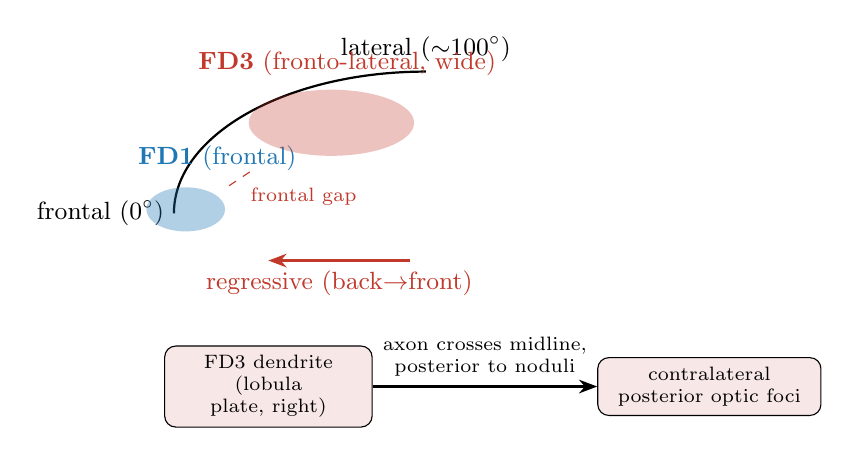
\begin{tikzpicture}[font=\small,>=Stealth]
  % visual field arc (one eye), frontal at left, lateral at right
  \draw[thick] (0,0) arc (180:90:3.2 and 1.8);
  \node[anchor=east] at (0,0) {frontal ($0^\circ$)};
  \node[anchor=south] at (3.2,1.8) {lateral ($\sim$100$^\circ$)};
  % FD1 receptive field (frontal, narrow)
  \fill[fd1c,opacity=0.35] (0.15,0.05) ellipse (0.5 and 0.28);
  \node[fd1c] at (0.55,0.7) {\textbf{FD1} (frontal)};
  % FD3 receptive field (fronto-lateral, wide) with a frontal gap
  \fill[fd3c,opacity=0.30] (2.0,1.15) ellipse (1.05 and 0.42);
  \node[fd3c] at (2.2,1.9) {\textbf{FD3} (fronto-lateral, wide)};
  \draw[fd3c,dashed] (0.7,0.35) -- (1.0,0.55) node[midway,below right,fd3c]{\scriptsize frontal gap};
  % regressive (back-to-front) preferred motion arrow
  \draw[->,thick,fd3c] (3.0,-0.6) -- (1.2,-0.6) node[midway,below]{regressive (back$\to$front)};
  % heterolateral axon
  \node[draw,rounded corners,fill=fd3c!12,font=\scriptsize,align=center,text width=2.4cm]
        (lp) at (1.2,-2.2) {FD3 dendrite\\(lobula plate, right)};
  \node[draw,rounded corners,fill=fd3c!12,font=\scriptsize,align=center,text width=2.6cm]
        (pof) at (6.8,-2.2) {contralateral\\posterior optic foci};
  \draw[->,thick] (lp) -- node[above,midway,font=\scriptsize,align=center]
        {axon crosses midline,\\posterior to noduli} (pof);
\end{tikzpicture}
\caption{\textbf{The FD3 cell and what distinguishes it.} Egelhaaf (1985, Part~II) defined four
figure-detection (FD) cells. FD3 is excited by \emph{regressive} (back-to-front) small-field
motion; its excitatory receptive field is \emph{fronto-lateral} (peak azimuth $40$--$50^\circ$,
half-width $\sim$$62^\circ$) and, uniquely among the FD cells, spares the most-frontal
$10$--$20^\circ$ (a ``frontal gap''). Like FD1 and FD4 it is a heterolateral ``noduli-group''
output element whose axon crosses the midline posterior to the noduli and terminates in the
contralateral posterior optic foci. This report maps FD3 onto the FlyWire cell type
\ttt{LPT42\_Nod4}.}\label{fig:concept}
\end{figure}


\section{The evidence}

We take FD3's defining properties one at a time: cell class, preferred motion, receptive-field position, small-field selectivity, output side, and cell shape. For each property we ask whether \ttt{LPT42\_Nod4} has the corresponding connectomic signature. Figure~\ref{fig:crosswalk} previews the correspondence; the paragraphs that follow establish each line of it.

\begin{figure}[H]\centering
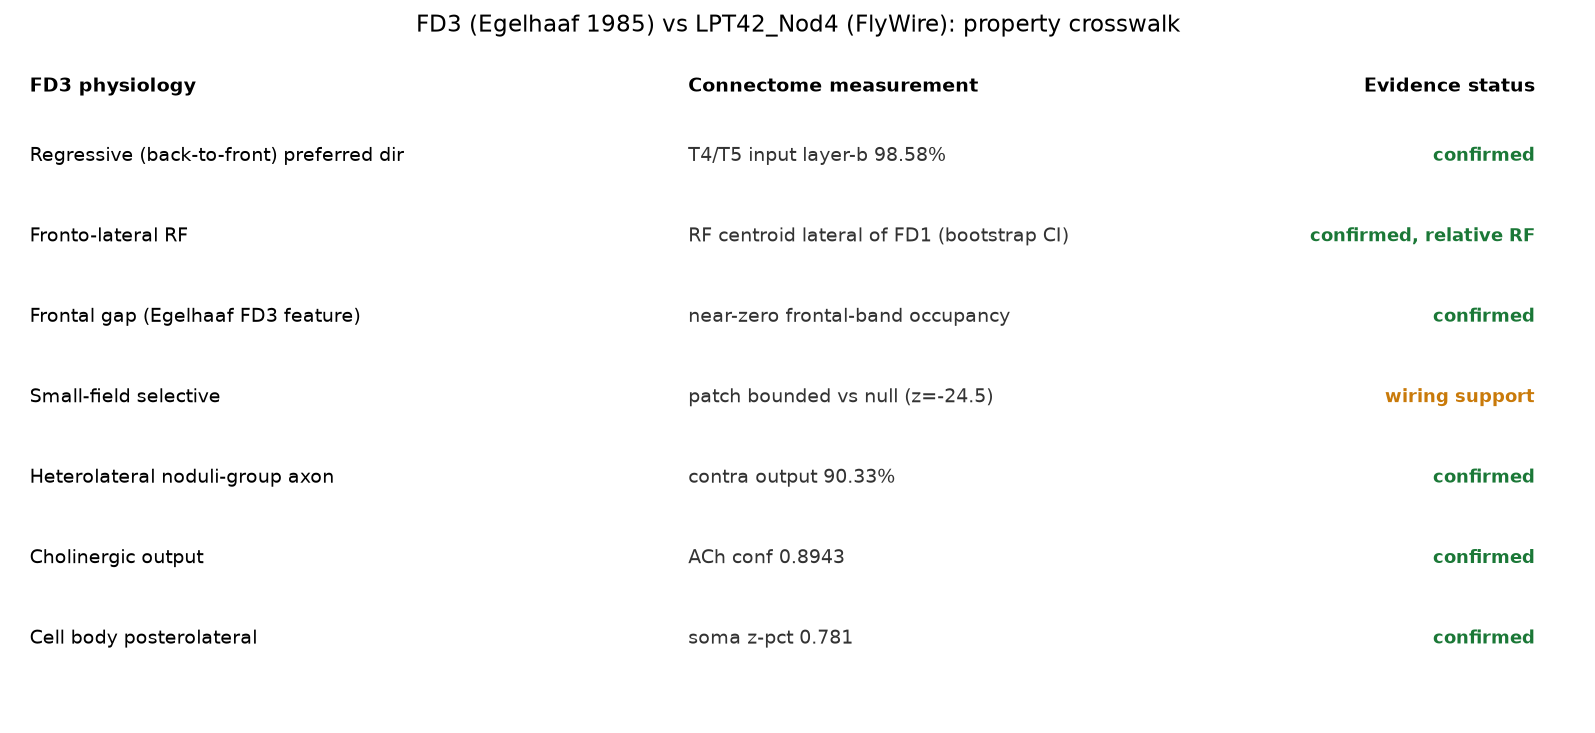
\includegraphics[width=\textwidth]{figures/fd3_crosswalk.png}
\caption{\textbf{FD3's properties and their connectome counterparts.} Each defining property of Egelhaaf's FD3 cell (left), and the matching measurement for \ttt{LPT42\_Nod4} (right), with caveated properties marked in the text.}\label{fig:crosswalk}
\end{figure}


\paragraph{It is an excitatory output cell, one per side.} \ttt{LPT42\_Nod4} is a pair of cells, one in each hemisphere, classified as a visual output neuron. It releases the excitatory transmitter acetylcholine, assigned with high confidence (0.8943) for both cells. This is consistent with an FD cell that sends figure signals to downstream circuits, and is the same transmitter as the already-identified FD1 cell \ttt{Nod1}.

\paragraph{It prefers back-to-front motion.} The fly computes motion in four separate channels, one for each cardinal direction, kept in four physical layers of the lobula plate. A cell's preferred direction is therefore read from which layer its motion inputs come from. For \ttt{LPT42\_Nod4}, 98.58\% of that input comes from the back-to-front layer (Fig.~\ref{fig:layers}). It prefers regressive motion, matching the direction Egelhaaf reported for FD3 and opposing the front-to-back FD1 cell.

\begin{figure}[H]\centering
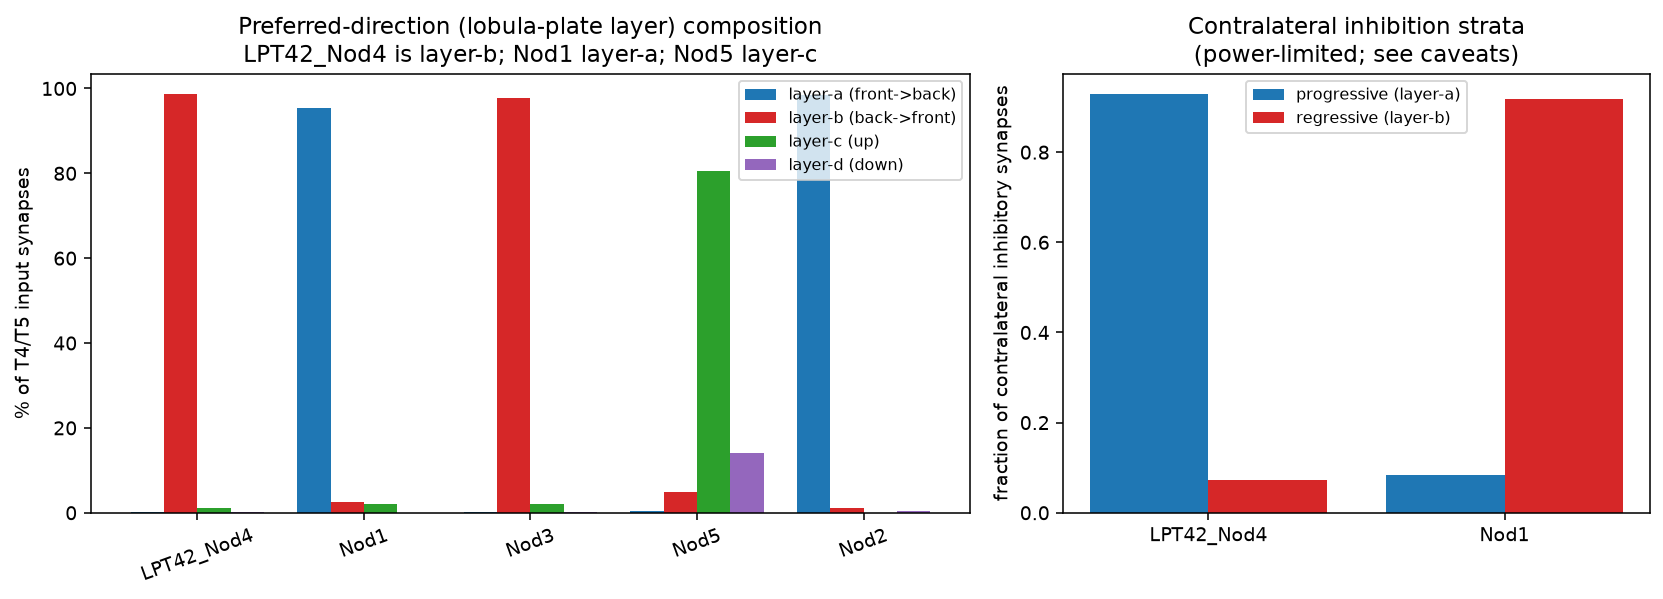
\includegraphics[width=\textwidth]{figures/fd3_layer_composition.png}
\caption{\textbf{Preferred direction.} (left) The share of each cell's motion input coming from the four directional layers. \ttt{LPT42\_Nod4} draws almost all of its input from the back-to-front layer (regressive, as FD3); \ttt{Nod1} from the front-to-back layer (FD1); \ttt{Nod5} from a vertical-motion layer. (right) The two directions of inhibition reaching the cell from the opposite eye.}\label{fig:layers}
\end{figure}


\paragraph{Its receptive field is lateral, with a gap at the front.} The part of the eye a cell sees is given by the retinal positions of the motion detectors that feed it. Compared with the frontal FD1 cell, measured in the same coordinate frame so the comparison needs no conversion into degrees, the inputs of \ttt{LPT42\_Nod4} sit clearly off to the side, by a margin larger than the measurement uncertainty, for both the left and the right cell (Fig.~\ref{fig:rf}a). It nearly avoids the most frontal part of the eye that FD1 fills (it covers about 2--3\% of that frontal zone, against about 60\% for FD1): this is the ``frontal gap'' that Egelhaaf singled out as unique to FD3 among all four FD cells (Fig.~\ref{fig:rf}b).

\paragraph{It responds to small objects, not the whole scene.} The defining behaviour of an FD cell is a stronger response to a small moving figure than to motion of the whole background. That requires the cell to gather its input from a compact patch of the visual field rather than spreading it everywhere. The input patch of \ttt{LPT42\_Nod4} is more concentrated than an in-degree matched random sample across the eye ($p=0.002$; Fig.~\ref{fig:rf}c). This provides wiring support for small-field selectivity; it is not a direct physiological measurement.

\begin{figure}[H]\centering
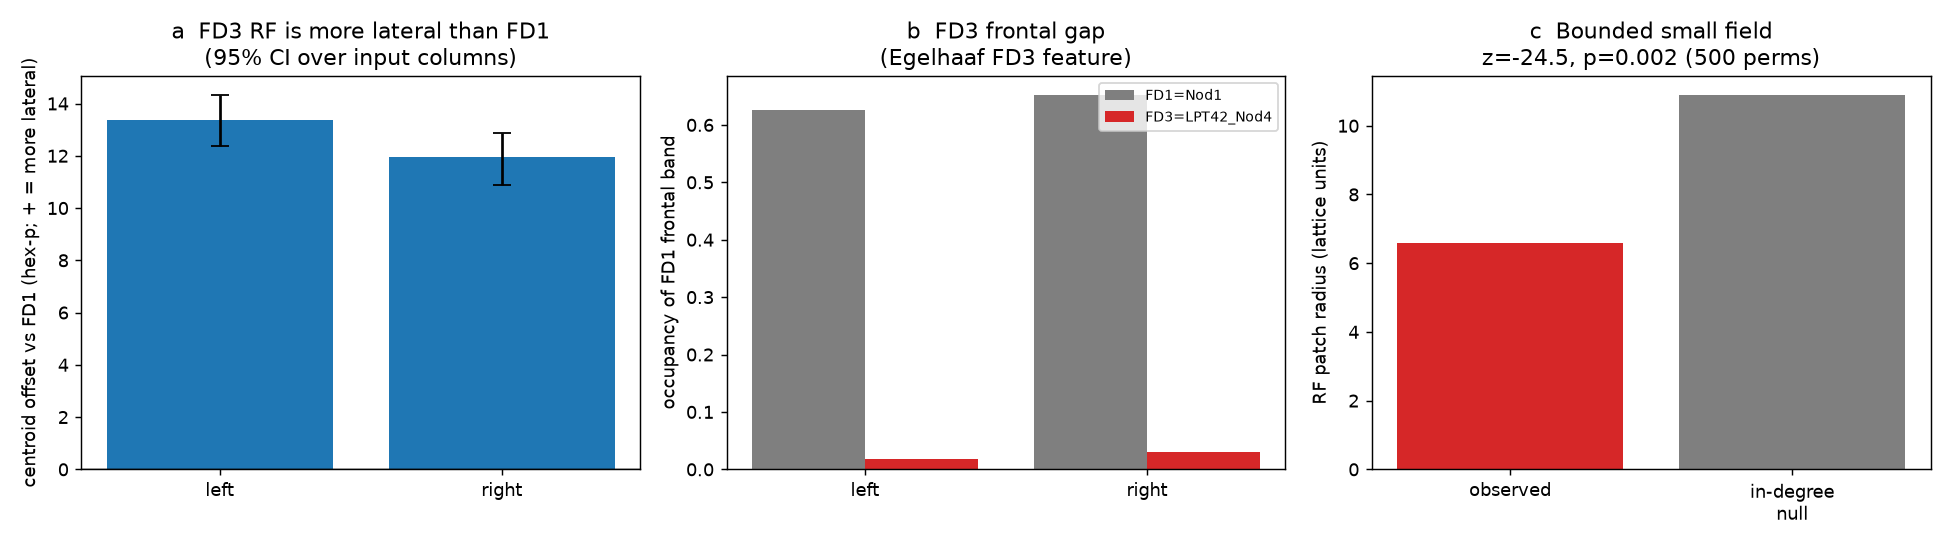
\includegraphics[width=\textwidth]{figures/fd3_rf_differential.png}
\caption{\textbf{The receptive field.} (a) For each cell, how far its input field sits to the side of the frontal FD1 field; the bars are well above zero with margin, on both sides. (b) How much of FD1's frontal zone each cell occupies: FD1 (grey) fills it, \ttt{LPT42\_Nod4} (red) leaves it almost empty, the frontal gap. (c) How tightly the cell's inputs cluster (red) compared with random sampling of the same number of inputs (grey): more concentrated, the wiring basis expected for small-field selectivity.}\label{fig:rf}
\end{figure}


\paragraph{Its axon crosses to the other side of the brain.} Egelhaaf found that the FD3 axon does not stay in the eye it serves: it crosses the brain's midline and ends on the opposite side. The connectome shows the same sidedness: 90.33\% of this cell's output synapses are on the opposite side of the brain from the cell itself, the signature of a cell that sends its signal across the midline, as FD3 (and FD1 and FD4) do (Fig.~\ref{fig:placement}).

\paragraph{Its cell body lies where Egelhaaf placed it.} Egelhaaf located the FD3 cell body toward the back and side of the central brain. The two \ttt{LPT42\_Nod4} cell bodies sit in that posterior and lateral region: one on each side of the midline, among the rearmost 78\% of visual output cells, right beside the cell bodies of the FD1 cell, and far behind the feedback cells that inhibit them (Fig.~\ref{fig:placement}).

\begin{figure}[H]\centering
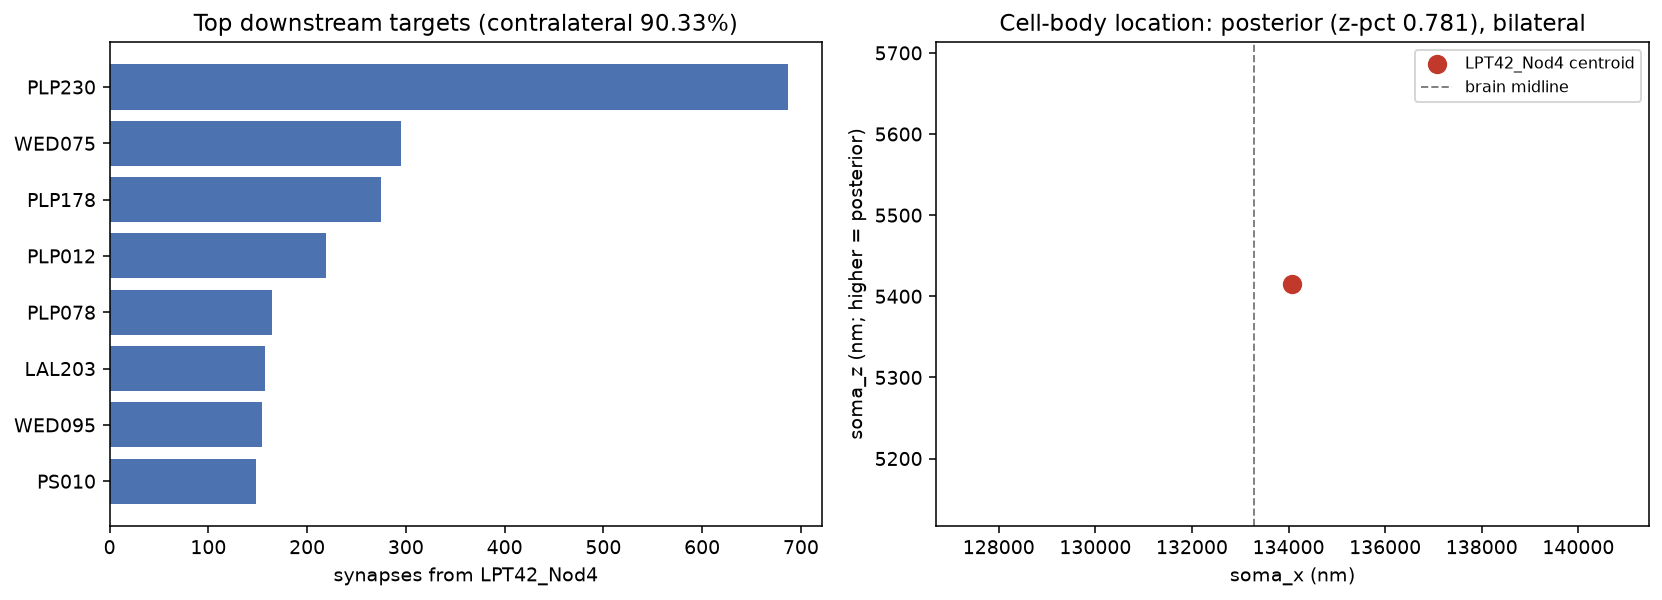
\includegraphics[width=\textwidth]{figures/fd3_circuit_placement.png}
\caption{\textbf{Where the cell sends its signal, and where its body sits.} (left) The main downstream targets of \ttt{LPT42\_Nod4}, the great majority on the opposite side of the brain. (right) The two cell bodies, sitting toward the back of the brain and one on each side of the midline.}\label{fig:placement}
\end{figure}


\paragraph{The shape of the cell.} We reconstruct each cell's branching skeleton from its three-dimensional shape in the connectome (right: 36744, left: 35808) and separate it into the dendrite, where the cell receives its inputs, and the axon, where it sends its outputs; the dendrite spans the full top-to-bottom (dorso-ventral) extent of the motion-processing layer ($\sim$155.0~$\mu$m, matching Egelhaaf's description), and its axon is shifted to the opposite side of the brain from its dendrite, ending roughly twice as close to the target region as the dendrite is. This is consistent with the heterolateral, midline-crossing axon Egelhaaf described for FD3 (Fig.~\ref{fig:morph}).

\begin{figure}[H]\centering
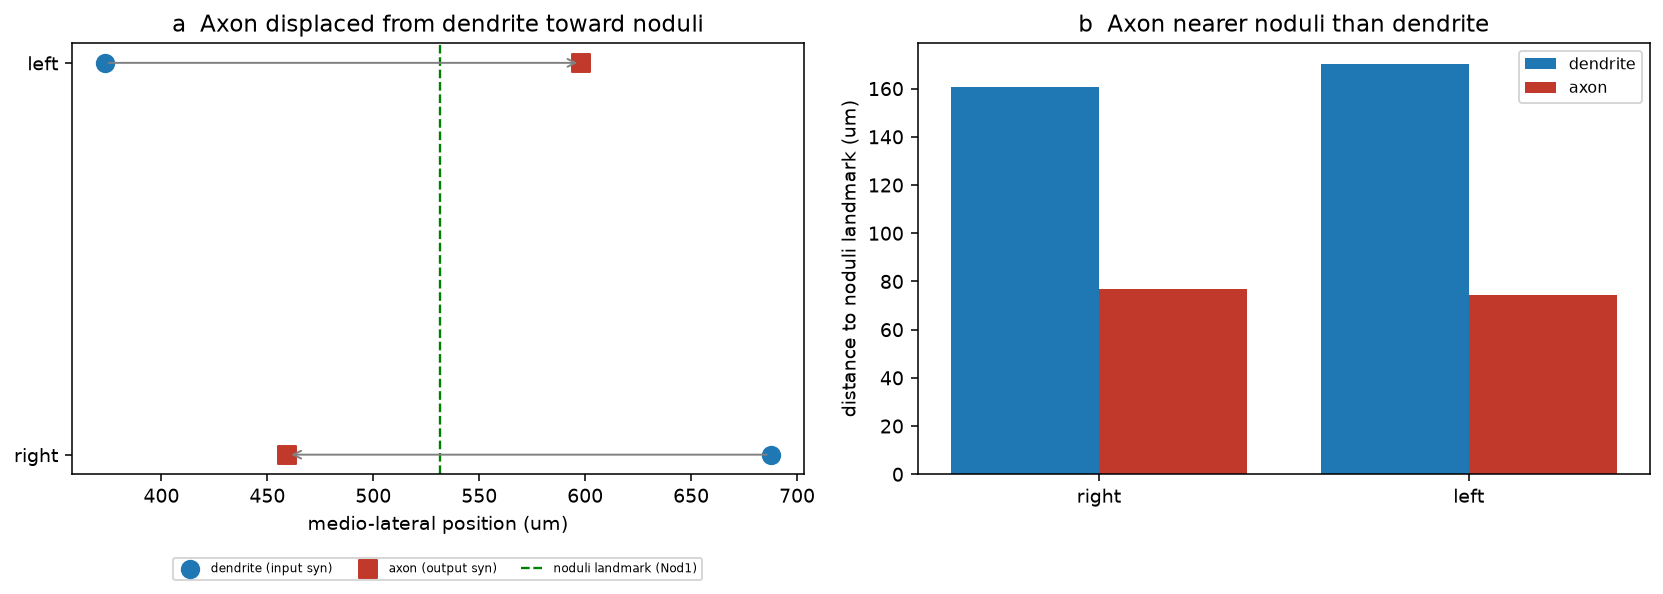
\includegraphics[width=\textwidth]{figures/fd3_morphology.png}
\caption{\textbf{The shape of the cell.} Reconstructed skeletons of the two \ttt{LPT42\_Nod4} cells. (a) For each cell, the output (axonal) part of the arbor, in red, sits to one side of the input (dendritic) part, in blue, shifted toward the region where Egelhaaf's FD3 axon terminates, in green. This is the expected geometry for a cell whose axon crosses the brain's midline. (b) The output arbor lies closer to that target region than the input arbor does.}\label{fig:morph}
\end{figure}


\paragraph{No other cell type matches FD3 as well.} The strongest form of the argument compares every candidate cell type against all four FD cells at once. For each, we score how many of the defining FD features it shares: preferred direction, the lateral field with a frontal gap, and the crossing axon. \ttt{LPT42\_Nod4} matches FD3 on every count, more closely than any other candidate matches FD3, and more closely than \ttt{LPT42\_Nod4} matches any other FD cell (Fig.~\ref{fig:heatmap}). The identification is therefore specific within the screened Nod/LPT candidate set.

\begin{figure}[H]\centering

\includegraphics[width=\textwidth]{figures/fd3_family_heatmap.png}
\caption{\textbf{The match is specific.} Each candidate cell type (columns) scored against each of the four FD cells (rows) by how many defining features it shares (0--3). \ttt{LPT42\_Nod4} (outlined) is the strongest match for FD3, and FD3 is its strongest match in return.}\label{fig:heatmap}
\end{figure}


\paragraph{The neighbouring cell types are not FD3.} An identification is only meaningful if the same measurements distinguish \ttt{LPT42\_Nod4} from the cells most easily confused with it. They do. \ttt{Nod1} prefers front-to-back motion and has a frontal field, which marks it as FD1 rather than FD3. \ttt{Nod2} is inhibitory (GABA-releasing) rather than an excitatory output cell. \ttt{Nod3} also prefers back-to-front motion but its output stays on the same side of the brain rather than crossing the midline. \ttt{Nod5} responds to vertical rather than horizontal motion and feeds the wide-field inhibitory cells, marking it as part of the feedback machinery rather than a figure-detection output. Applying the full set of FD3 measurements to any of these cells fails to reproduce the FD3 signature.

\paragraph{The provenance is explicit.} The primary numbers come from the \ttt{offline} track. The v630 cross-version check is not claimed in this artifact because v630 cross-check is live-only. The identity evidence still requires agreement between the left and right \ttt{LPT42\_Nod4} cells and comparison against neighbouring Nod/LPT candidates (Fig.~\ref{fig:replication}).

\paragraph{The result is the same regardless of analysis choices.} The conclusions are unchanged when the thresholds that define ``lateral'', ``frontal gap'' and ``crosses the midline'' are varied across their reasonable ranges, and when the random-sampling steps are repeated with different seeds, so no finding rests on a particular cutoff (Fig.~\ref{fig:replication}).

\begin{figure}[H]\centering
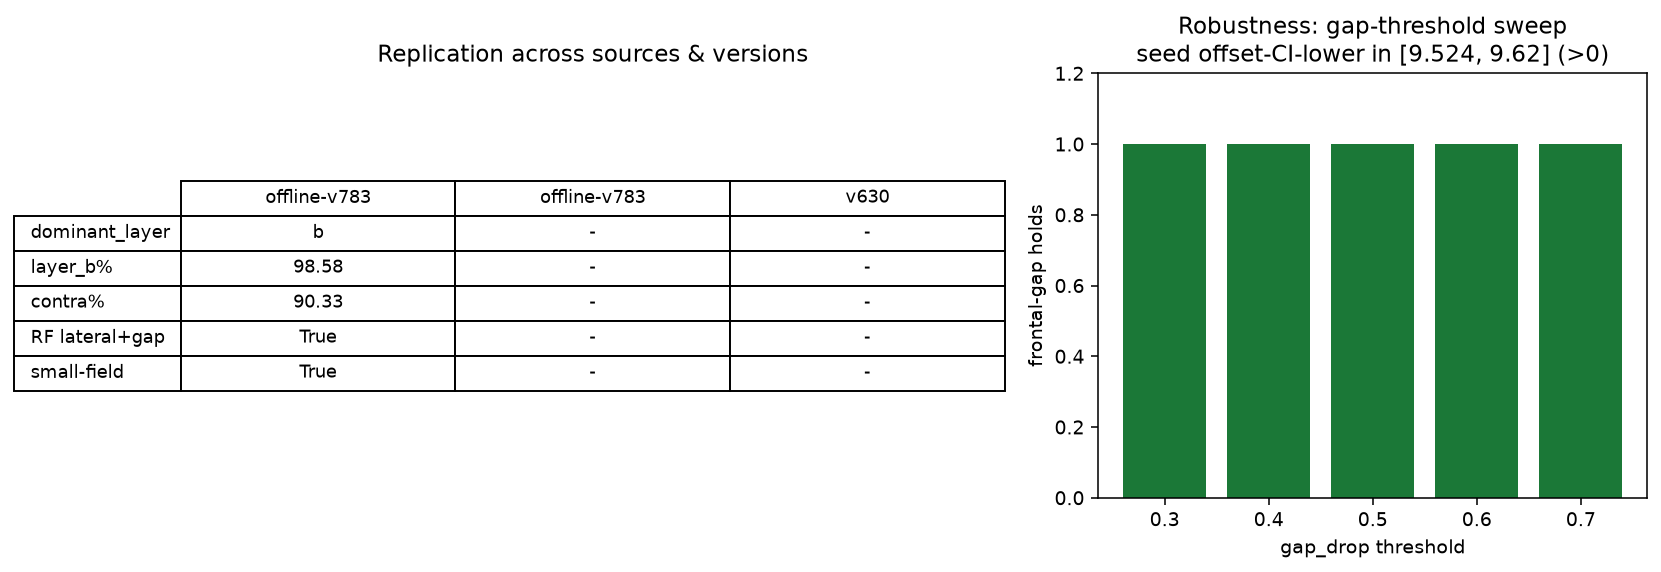
\includegraphics[width=\textwidth]{figures/fd3_replication_robustness.png}
\caption{\textbf{Stability of the findings.} (left) Available provenance for the defining FD3 measurements; unavailable cross-version checks are marked as missing rather than inferred. (right) The frontal gap persists as its defining threshold is varied, and the lateral-displacement estimate stays positive across resampling seeds.}\label{fig:replication}
\end{figure}


\section{The evidence at a glance}

Table~\ref{tab:evidence} collects the defining FD3 properties next to the connectome measurement that establishes it for \ttt{LPT42\_Nod4}. Each row is developed in the corresponding part of the Results above.

\begin{table}[H]\centering\footnotesize\caption{Each defining property of Egelhaaf's FD3 cell and the matching measurement for the FlyWire cell type \ttt{LPT42\_Nod4}.}\label{tab:evidence}

\renewcommand{\arraystretch}{1.25}
\setlength{\tabcolsep}{3pt}
\begin{longtable}{@{}>{\raggedright\arraybackslash}p{0.24\textwidth} >{\raggedright\arraybackslash}p{0.28\textwidth} >{\raggedright\arraybackslash}p{0.38\textwidth}@{}}
\toprule \textbf{FD3 property} & \textbf{What Egelhaaf reported} & \textbf{What we find for \ttt{LPT42\_Nod4}} \\\midrule\endhead
Prefers regressive (back-to-front) motion & Egelhaaf: FD3 excited by regressive motion & 98.58\% of its motion (T4/T5) input comes from the back-to-front lobula-plate layer \\
Excitatory output (cholinergic) & FD cells are excitatory output neurons & acetylcholine, assigned with 0.8943 confidence for both cells \\
Receptive field lateral, not frontal & Egelhaaf: FD3 field peaks at $40$--$50^\circ$, away from the front & its input field sits $\sim$12--13 columns lateral of the frontal FD1 cell, on both sides \\
Frontal gap (unique to FD3) & Egelhaaf: FD3 alone is not excited in the most-frontal field & occupies $\sim$2--3\% of the frontal zone that FD1 fills (vs $\sim$60\% for FD1) \\
Small-object selective & FD cells prefer small figures to wide-field motion & pools a bounded retinotopic patch below the in-degree matched null ($z=-24.5$, $p=0.002$) \\
Heterolateral output axon & Egelhaaf: axon crosses to the opposite (contralateral) side & 90.33\% of output synapses on the opposite side \\
Cell body posterior and lateral & Egelhaaf: cell body in the posterior lateral protocerebrum & both somata in the posterior 78th percentile, bilateral, beside the FD1 cell bodies \\
Dendrite spans the full dorso-ventral field & Egelhaaf: dendrite covers the entire dorso-ventral extent & 155.0~$\mu$m span in the reconstructed skeleton \\
Best and unique match for FD3 & the identification must be specific & best match for FD3 among 5 candidates, and FD3 is its own best match (by a clear margin) \\
Provenance is explicit & the result should not depend on an unreported dataset & primary track: \ttt{offline}; v630 not available in this artifact \\
\bottomrule\end{longtable}
\renewcommand{\arraystretch}{1.0}
\setlength{\tabcolsep}{6pt}

\end{table}

\section{What the data can and cannot settle}

Three points deserve to be stated plainly so the strength of the identification is not overstated. \textbf{There are only two cells.} \ttt{LPT42\_Nod4} is a single bilateral pair -- one cell per side -- and this is simply how many the fly has, so the result cannot be averaged over a large sample. Its robustness comes instead from the left and right cell agreeing independently, from comparison against neighbouring candidate types, and from statistical resampling of the thousands of synapses that make up each cell. \textbf{Absolute visual angle is approximate.} Egelhaaf measured the receptive field in degrees of visual angle; the connectome gives positions on the eye's lattice, and converting one to the other is only approximate (to within about $16.0^\circ$). For this reason the receptive-field argument is built on a \emph{relative} comparison to the frontal FD1 cell, which needs no such conversion; the absolute degree figures are reported only as a consistency check. \textbf{Fine branch-level anatomy is at the limit of the reconstruction.} The cell's overall shape -- the extent of its dendrite and the side its axon projects to -- is recovered clearly, both from its synapse positions and from its reconstructed skeleton, and the two agree. Still finer details of the arbor are at the resolution limit of the automated reconstruction and are not pressed further here.

\section{Methods and provenance}

\textbf{Connectomes.} FlyWire FAFB materialization v783 (\ttt{synapses\_nt\_v1}, no cleft threshold) on the \ttt{offline} track as the primary source for the numbers in this report. A v630 cross-version check is not claimed here because v630 cross-check is live-only. Neuron annotations (cell type, side, super-class, neurotransmitter and confidence, soma coordinates) are the Schlegel/Codex tables. \textbf{Preferred direction} is the synapse-weighted T4/T5 lobula-plate layer composition (layer$\to$direction after Fischbach \& Dittrich and Maisak et al.~\cite{fd1989,maisak2013}). \textbf{Receptive field}: T4/T5 inputs carry hex-lattice (p,q) coordinates; the differential test compares the synapse-weighted centroid, half-width and frontal-band occupancy against the FD1=\ttt{Nod1} anchor, with a 2000-sample within-cell bootstrap and a 500-permutation in-degree null; the axis convention is pinned by a self-test requiring the known-frontal FD1 anchor to land frontal. \textbf{Family screen}: a binary feature-match score over all Nod/LPT \ttt{visual\_projection} types. \textbf{Reproducibility}: all randomness is seeded (12345, plus a 5-seed stability set). The report is built from the verification JSON by the FD3 report CLI. Primary track for the numbers herein: \ttt{offline}.

\clearpage\part{Inputs: what drives FD3}

\textbf{Summary.}\quad The figure-detection cell FD3 -- the cell type \ttt{LPT42\_Nod4} in the fly connectome -- signals a small object moving from back to front on one side of the visual field. This report follows the wiring that \emph{drives} it: from the photoreceptors of the eye, through the lamina and medulla, to the local motion detectors, and onto FD3's dendrite, together with the central cells and the inhibition from the other eye that shape its response. We find that FD3's measured T4/T5 motion input comes almost entirely from the back-to-front (regressive) motion channel -- 98.58\% of its detector input is that one channel -- carried by both the ON (\ttt{T4b}) and the OFF (\ttt{T5b}) detectors. Those detectors are themselves fed by the canonical columnar cascade (photoreceptors, lamina, and the ON/OFF medulla cells), which is present in the connectome and matches the literature. Importantly, motion is only about 25.1\% of FD3's total input: most of its input comes from neighbouring columnar projection sheets and from inhibitory cells, including contralateral inhibition driven by the opposite eye. Unlike the previously mapped FD1 cell, FD3 has no centrifugal gate and no front-to-back drive -- it is a parallel, oppositely-tuned arm of the figure-ground system, not a copy of FD1.

\section{From the eye to FD3}

A moving object is first transduced by the photoreceptors, split into ON and OFF channels in the lamina and medulla, and turned into local direction-of-motion signals by the \ttt{T4} (ON) and \ttt{T5} (OFF) cells of the lobula plate. Each \ttt{T4}/\ttt{T5} cell prefers one of four directions, sorted into four layers of the lobula plate: layer~a is front-to-back, layer~b is back-to-front, and layers c and d are up and down~\cite{maisak2013}. A figure-detection cell reads out this motion map. The companion identity report showed that FD3 reads the back-to-front (layer~b) map with a receptive field placed off to the side and a gap directly in front; the descending report followed FD3's output to the descending neurons. Here we extend the trace on the input side, naming the cells that feed FD3 and tracing the pathway back to the eye.

\section{The motion detectors that drive FD3}

Of FD3's input from the local motion detectors, 98.58\% comes from the back-to-front (layer~b) channel, the direction FD3 is excited by, and essentially none from the opposite direction. That layer~b drive is carried by \emph{both} kinds of detector: the ON detector \ttt{T4b} (1793 synapses) and the OFF detector \ttt{T5b} (1459 synapses), a roughly even ON/OFF mix. So FD3 pools back-to-front motion of both contrast polarities, supporting an object signal across contrast polarity.

\begin{figure}[H]\centering
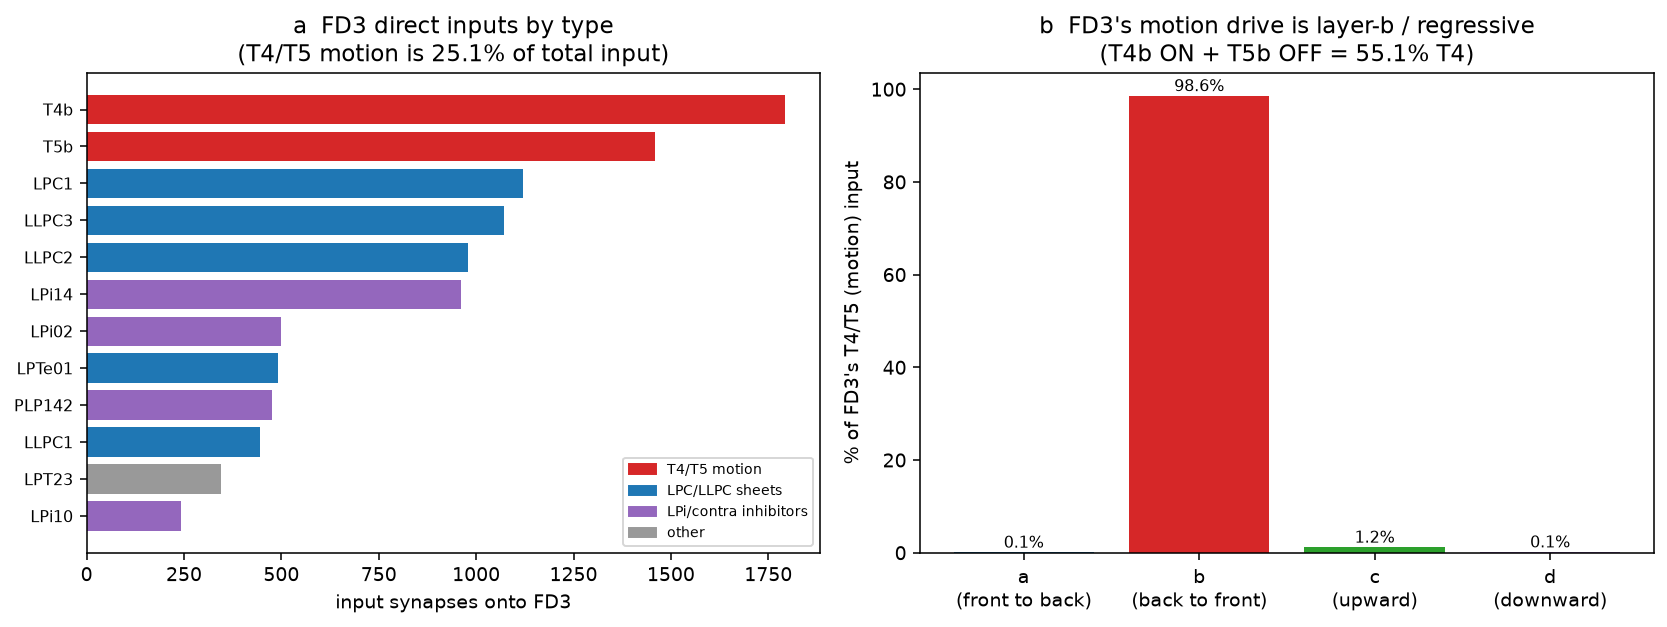
\includegraphics[width=\textwidth]{figures/fd3_input_census.png}
\caption{\textbf{What feeds FD3.} (a) FD3's direct inputs by cell type, coloured by class; the motion detectors (red) are only a minority of the total. (b) Within the motion input, almost all of it is the back-to-front (layer~b) channel, split between the ON and OFF detectors.}\label{fig:census}
\end{figure}


Following those detectors one step further back, the \ttt{T4b} cells that drive FD3 are themselves fed by the canonical ON medulla cells (C2, C3, Mi1, Mi4, Mi9, Tm3), and the \ttt{T5b} cells by the canonical OFF medulla cells (Tm1, Tm2, Tm4, Tm9); these in turn are fed by the lamina and, before it, the photoreceptors. The whole cascade from the eye to FD3's detectors is present in the connectome and matches published optic-lobe wiring. We show it as the afferent pathway below, marking which links we measure directly onto FD3 and which are the general column-to-column wiring of the optic lobe.

\begin{figure}[H]\centering
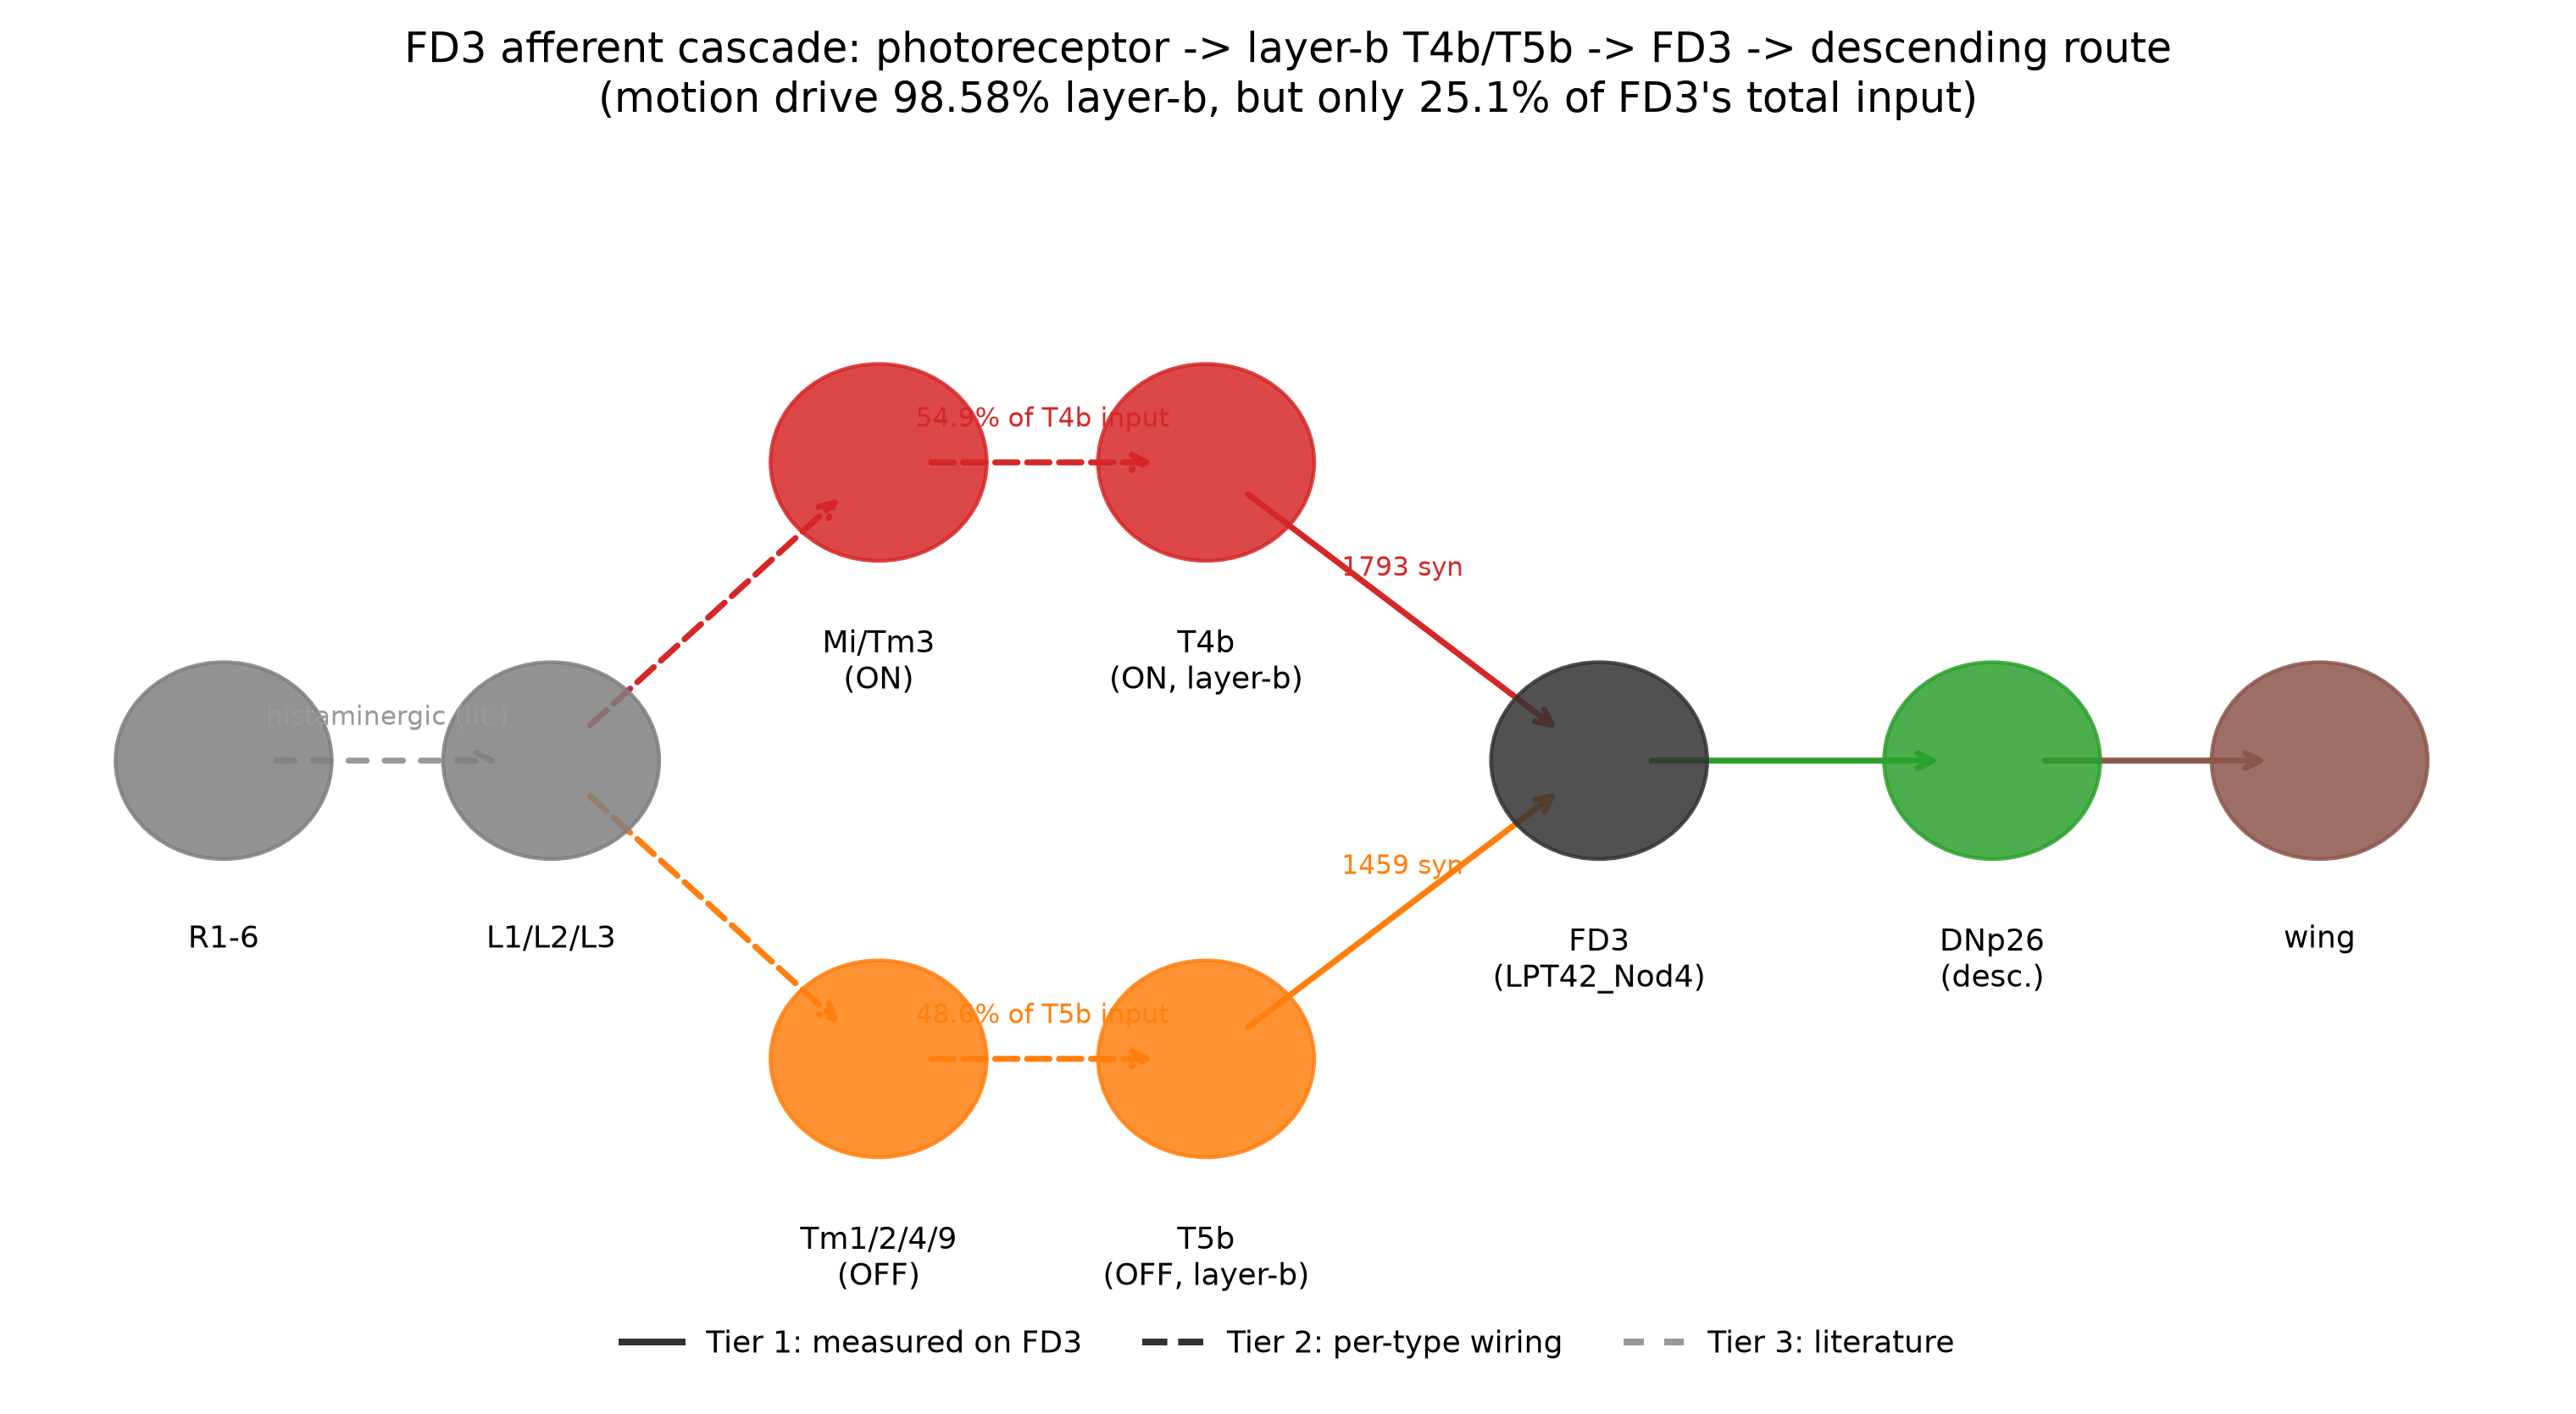
\includegraphics[width=\textwidth]{figures/fd3_afferent_cascade.png}
\caption{\textbf{The afferent cascade.} Photoreceptors $\rightarrow$ lamina $\rightarrow$ ON/OFF medulla $\rightarrow$ the back-to-front detectors \ttt{T4b}/\ttt{T5b} $\rightarrow$ FD3 $\rightarrow$ the steering neuron \ttt{DNp26} $\rightarrow$ wing. Solid links are measured on FD3 itself; dashed links are the standard column wiring measured cell-type by cell-type; the greyed link is the histaminergic front end known from physiology.}\label{fig:cascade}
\end{figure}


\section{Where the input lands}

Each motion detector looks at one point in the eye's field of view, so the set of detectors feeding FD3 draws out FD3's receptive field directly on the eye's lattice. Plotting those input columns shows FD3's field sitting off to the side, shifted away from straight ahead relative to the FD1 cell -- the lateral placement with a frontal gap that defines FD3.

\begin{figure}[H]\centering
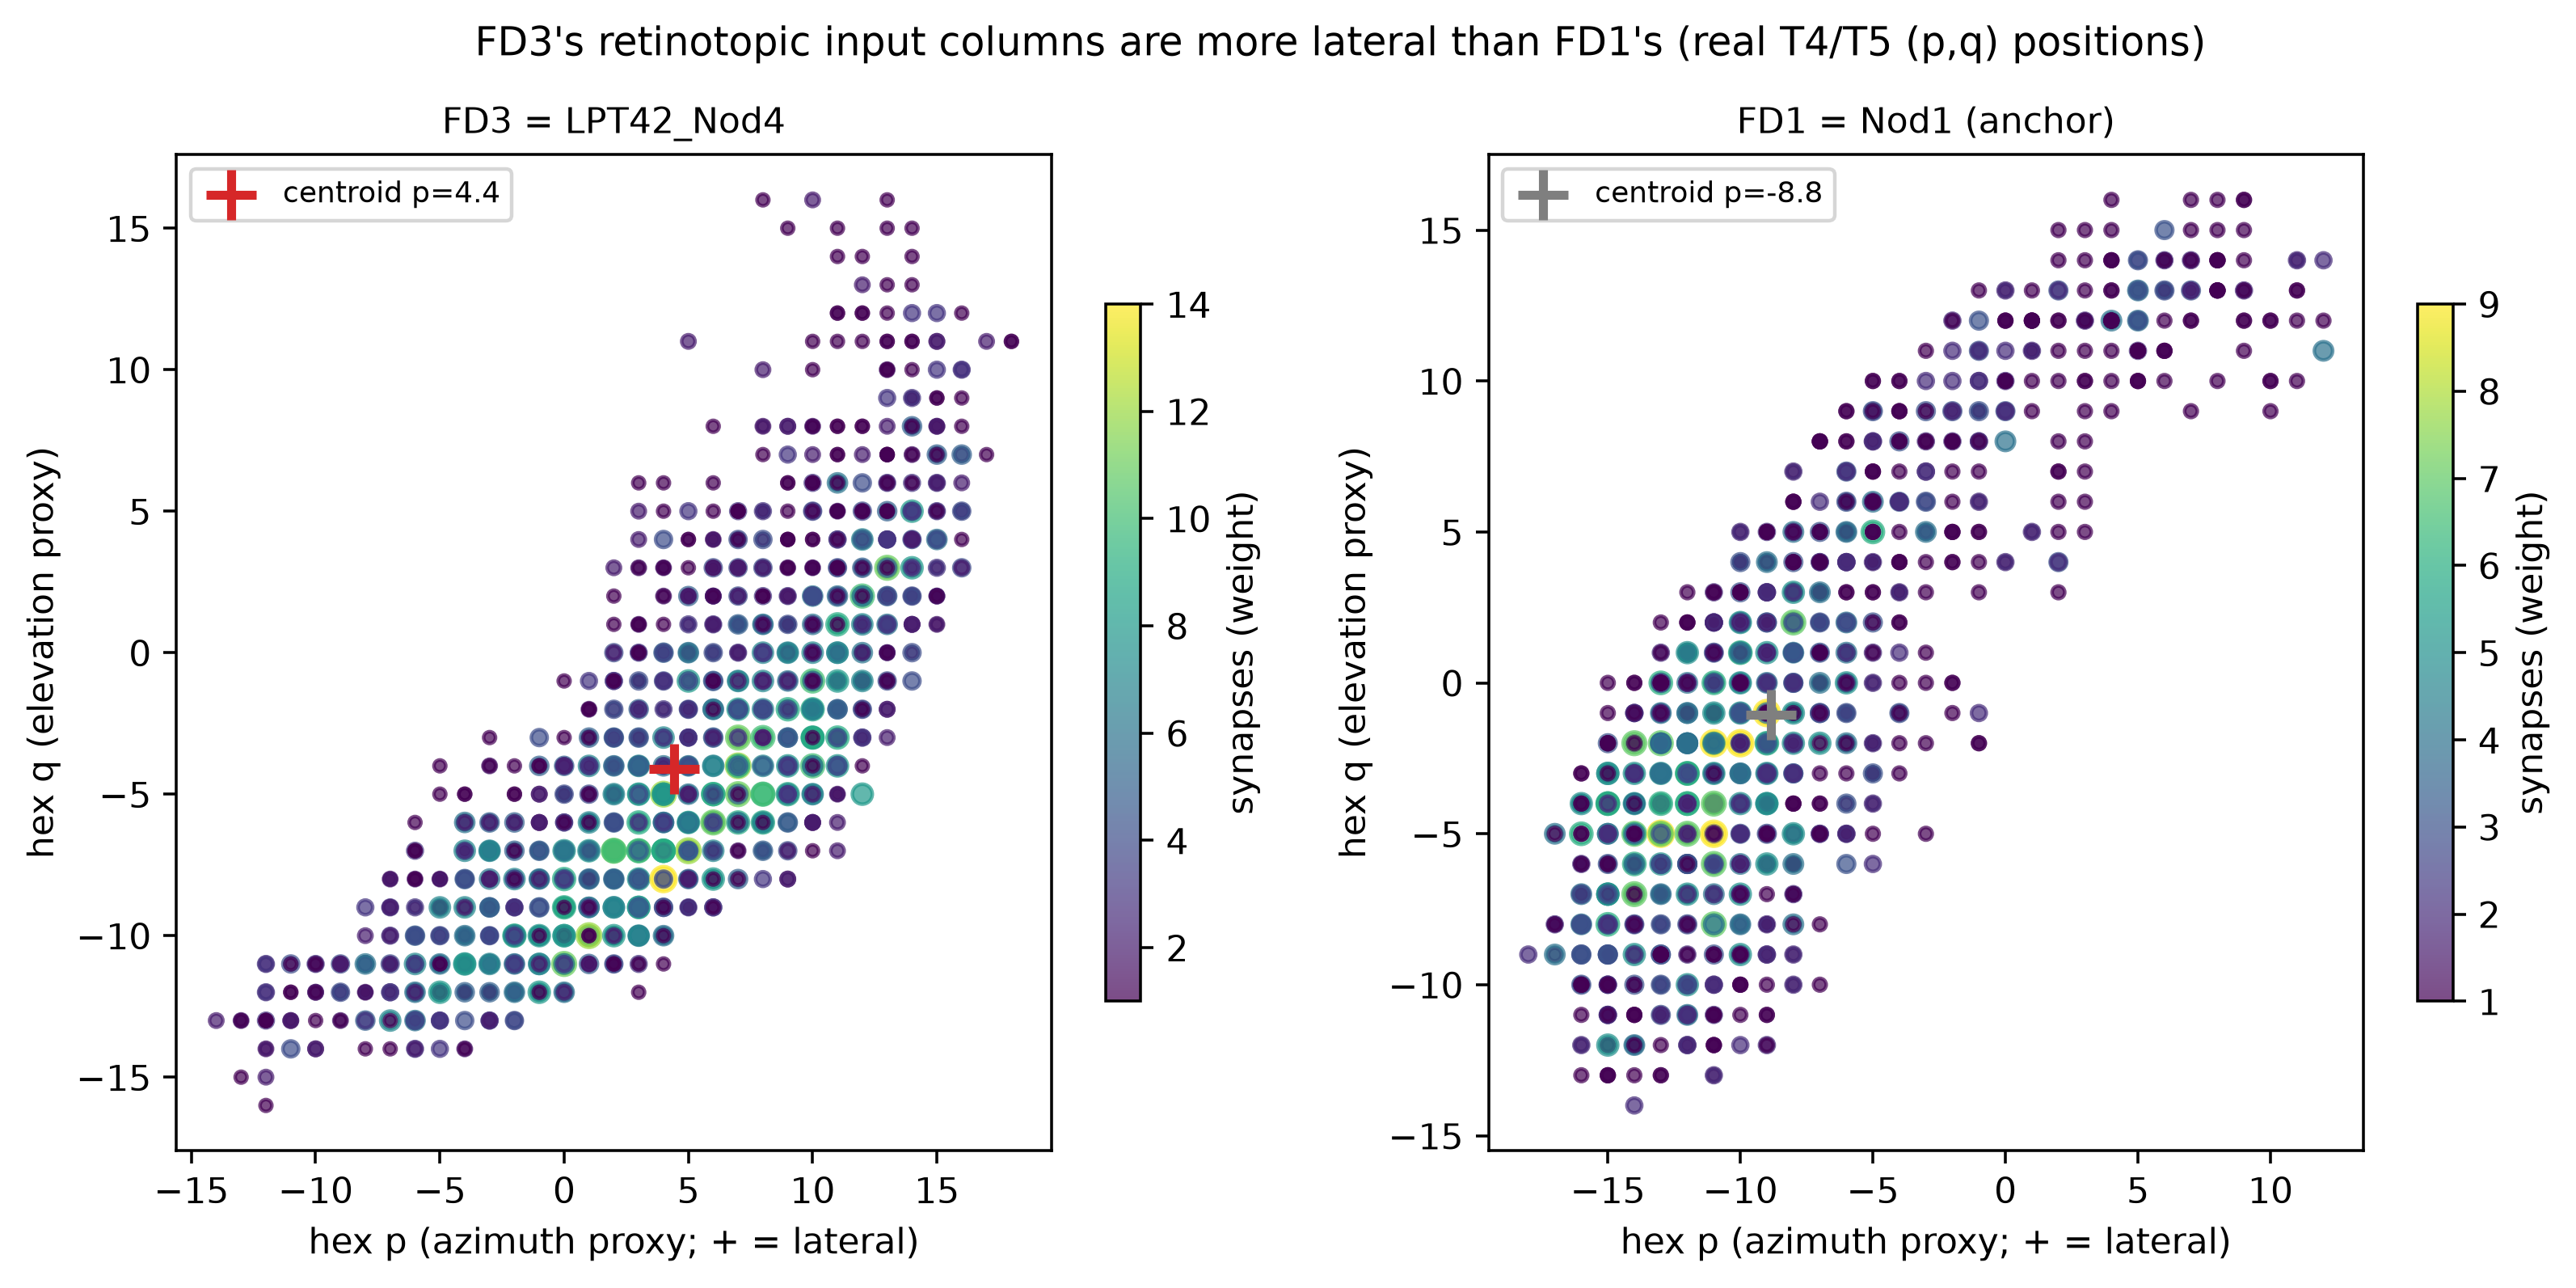
\includegraphics[width=\textwidth]{figures/fd3_input_hexmap.png}
\caption{\textbf{FD3's input in eye coordinates.} Every motion column feeding FD3 (left) and FD1 (right), placed on the eye's hexagonal lattice and shaded by synapse number. FD3's centre of mass sits further to the side.}\label{fig:hexmap}
\end{figure}


On the cell itself, the different kinds of input are not scattered at random: the motion detectors, the neighbouring projection sheets, and the inhibitory cells each contact characteristic parts of FD3's arbor. Rendering FD3's reconstructed shape with its input synapses marked shows where each class of input arrives.

\begin{figure}[p]\centering
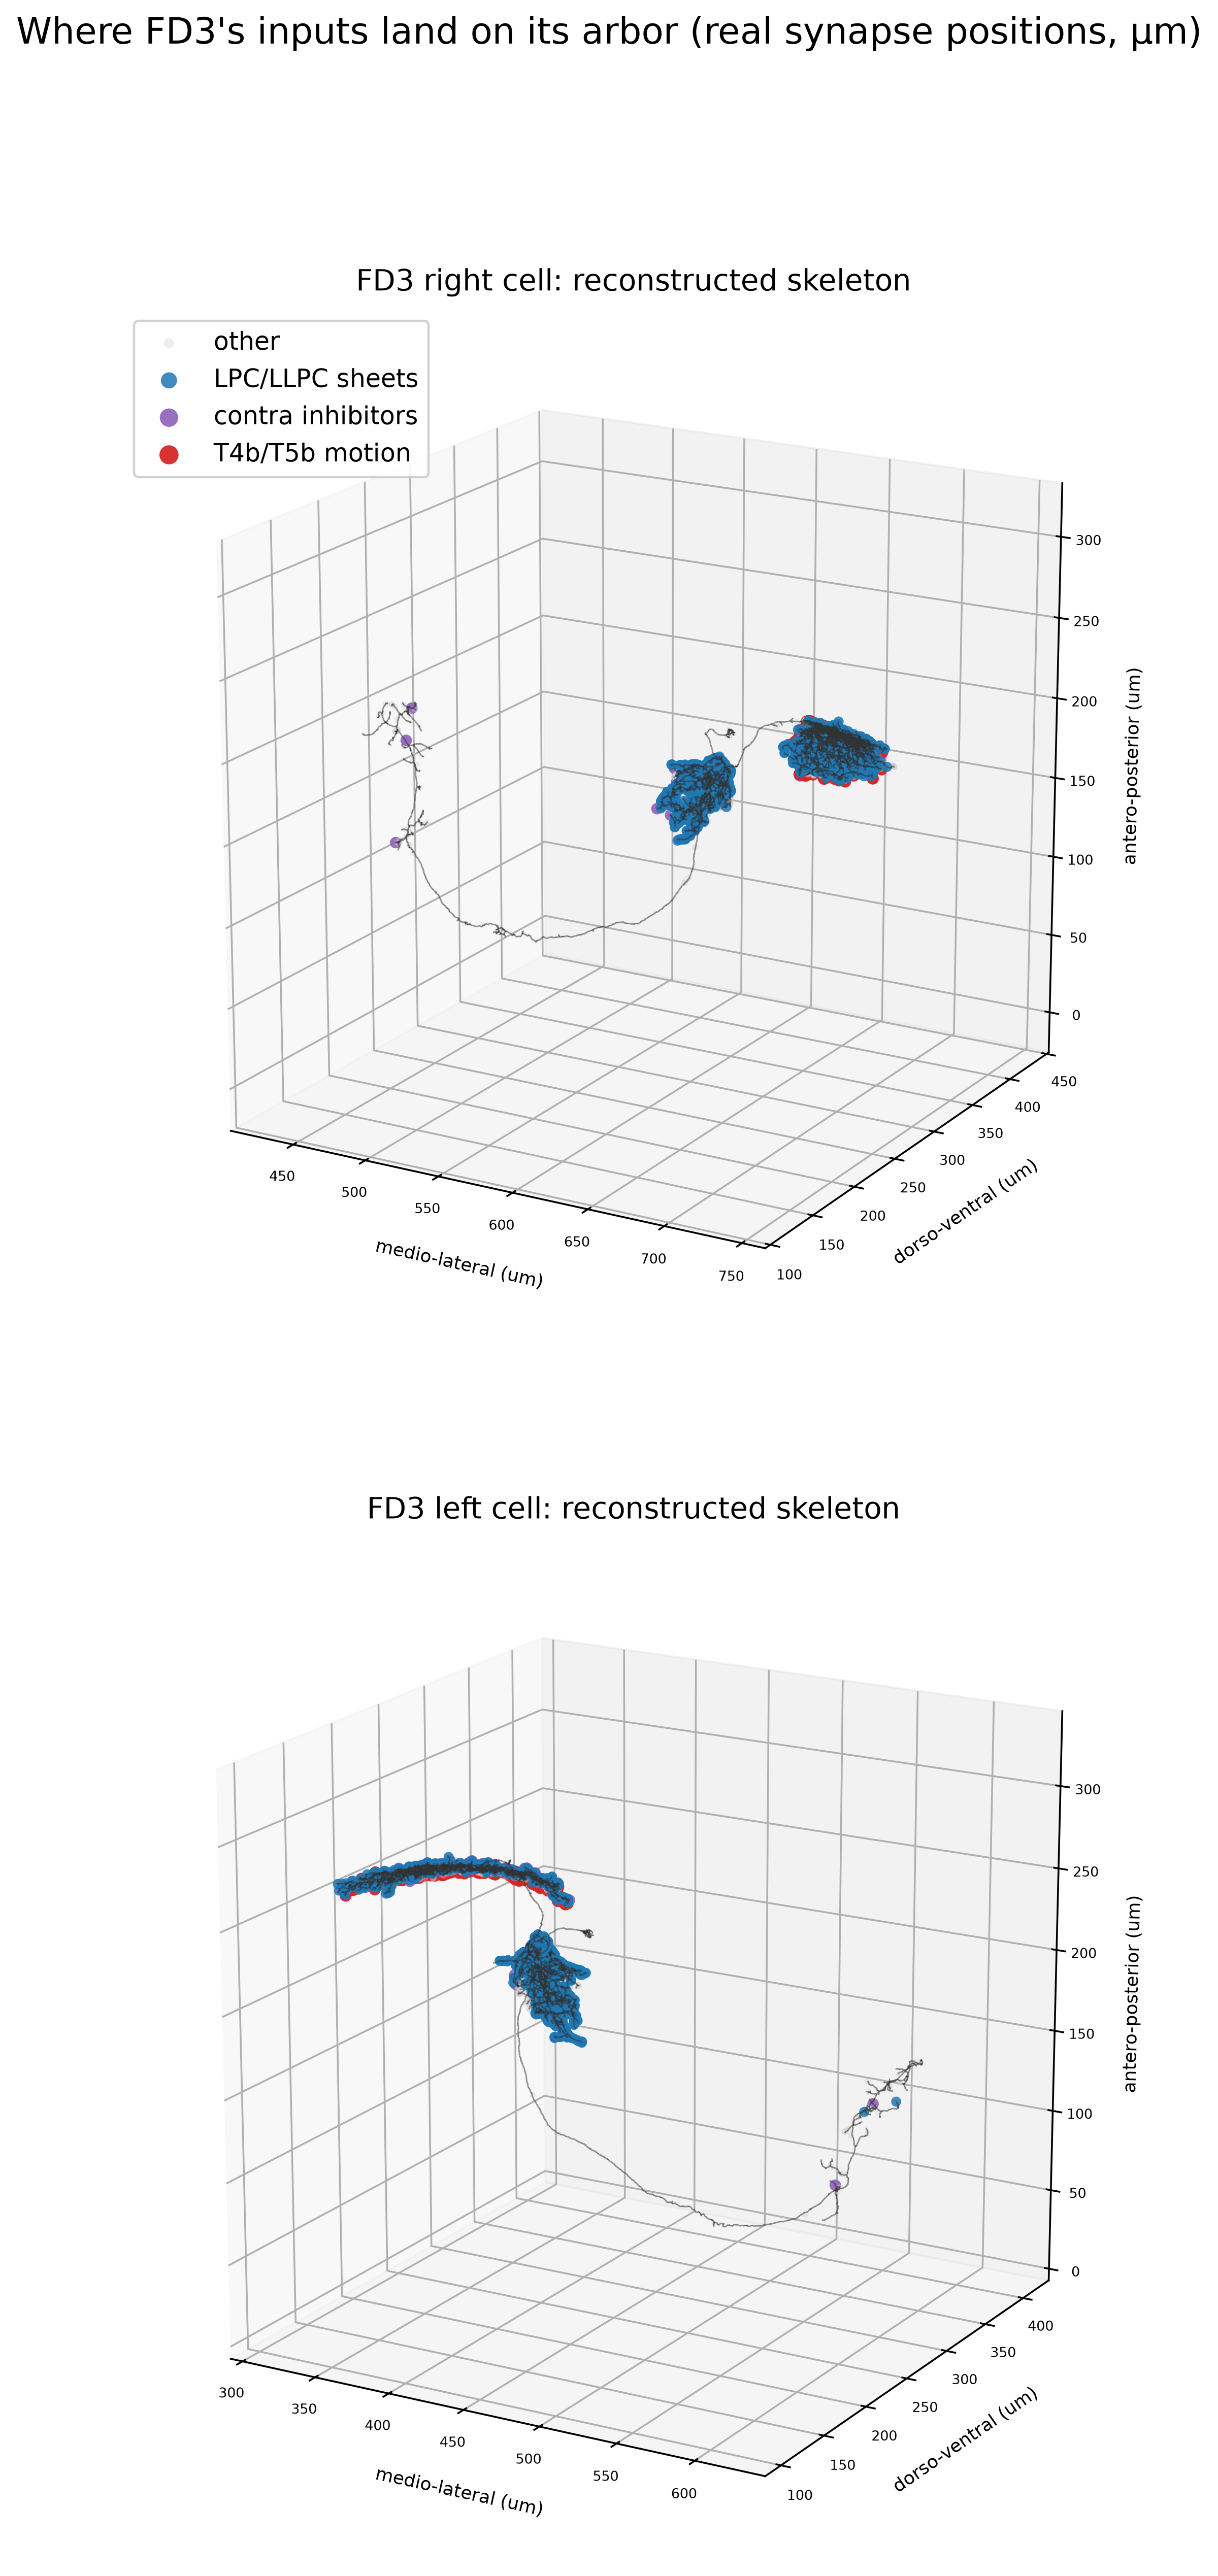
\includegraphics[width=\textwidth,height=0.86\textheight,keepaspectratio]{figures/fd3_arbor_inputs.png}
\caption{\textbf{Inputs on FD3's arbor.} Each FD3 cell's reconstructed shape (thin cable) with its input synapses drawn at their real positions and coloured by the class of cell they come from: back-to-front motion detectors (\ttt{T4b}/\ttt{T5b}), columnar projection sheets (\ttt{LPC}/\ttt{LLPC}), and contralateral inhibitors. The motion input clusters on the dendritic tuft in the lobula plate; the crossing axon carries the contralateral inhibitory contacts.}\label{fig:arbor}
\end{figure}


Seen alongside the cells it connects, FD3 sits anatomically between lobula-plate motion detectors and descending neurons that contact wing-steering motor systems.

\begin{figure}[p]\centering
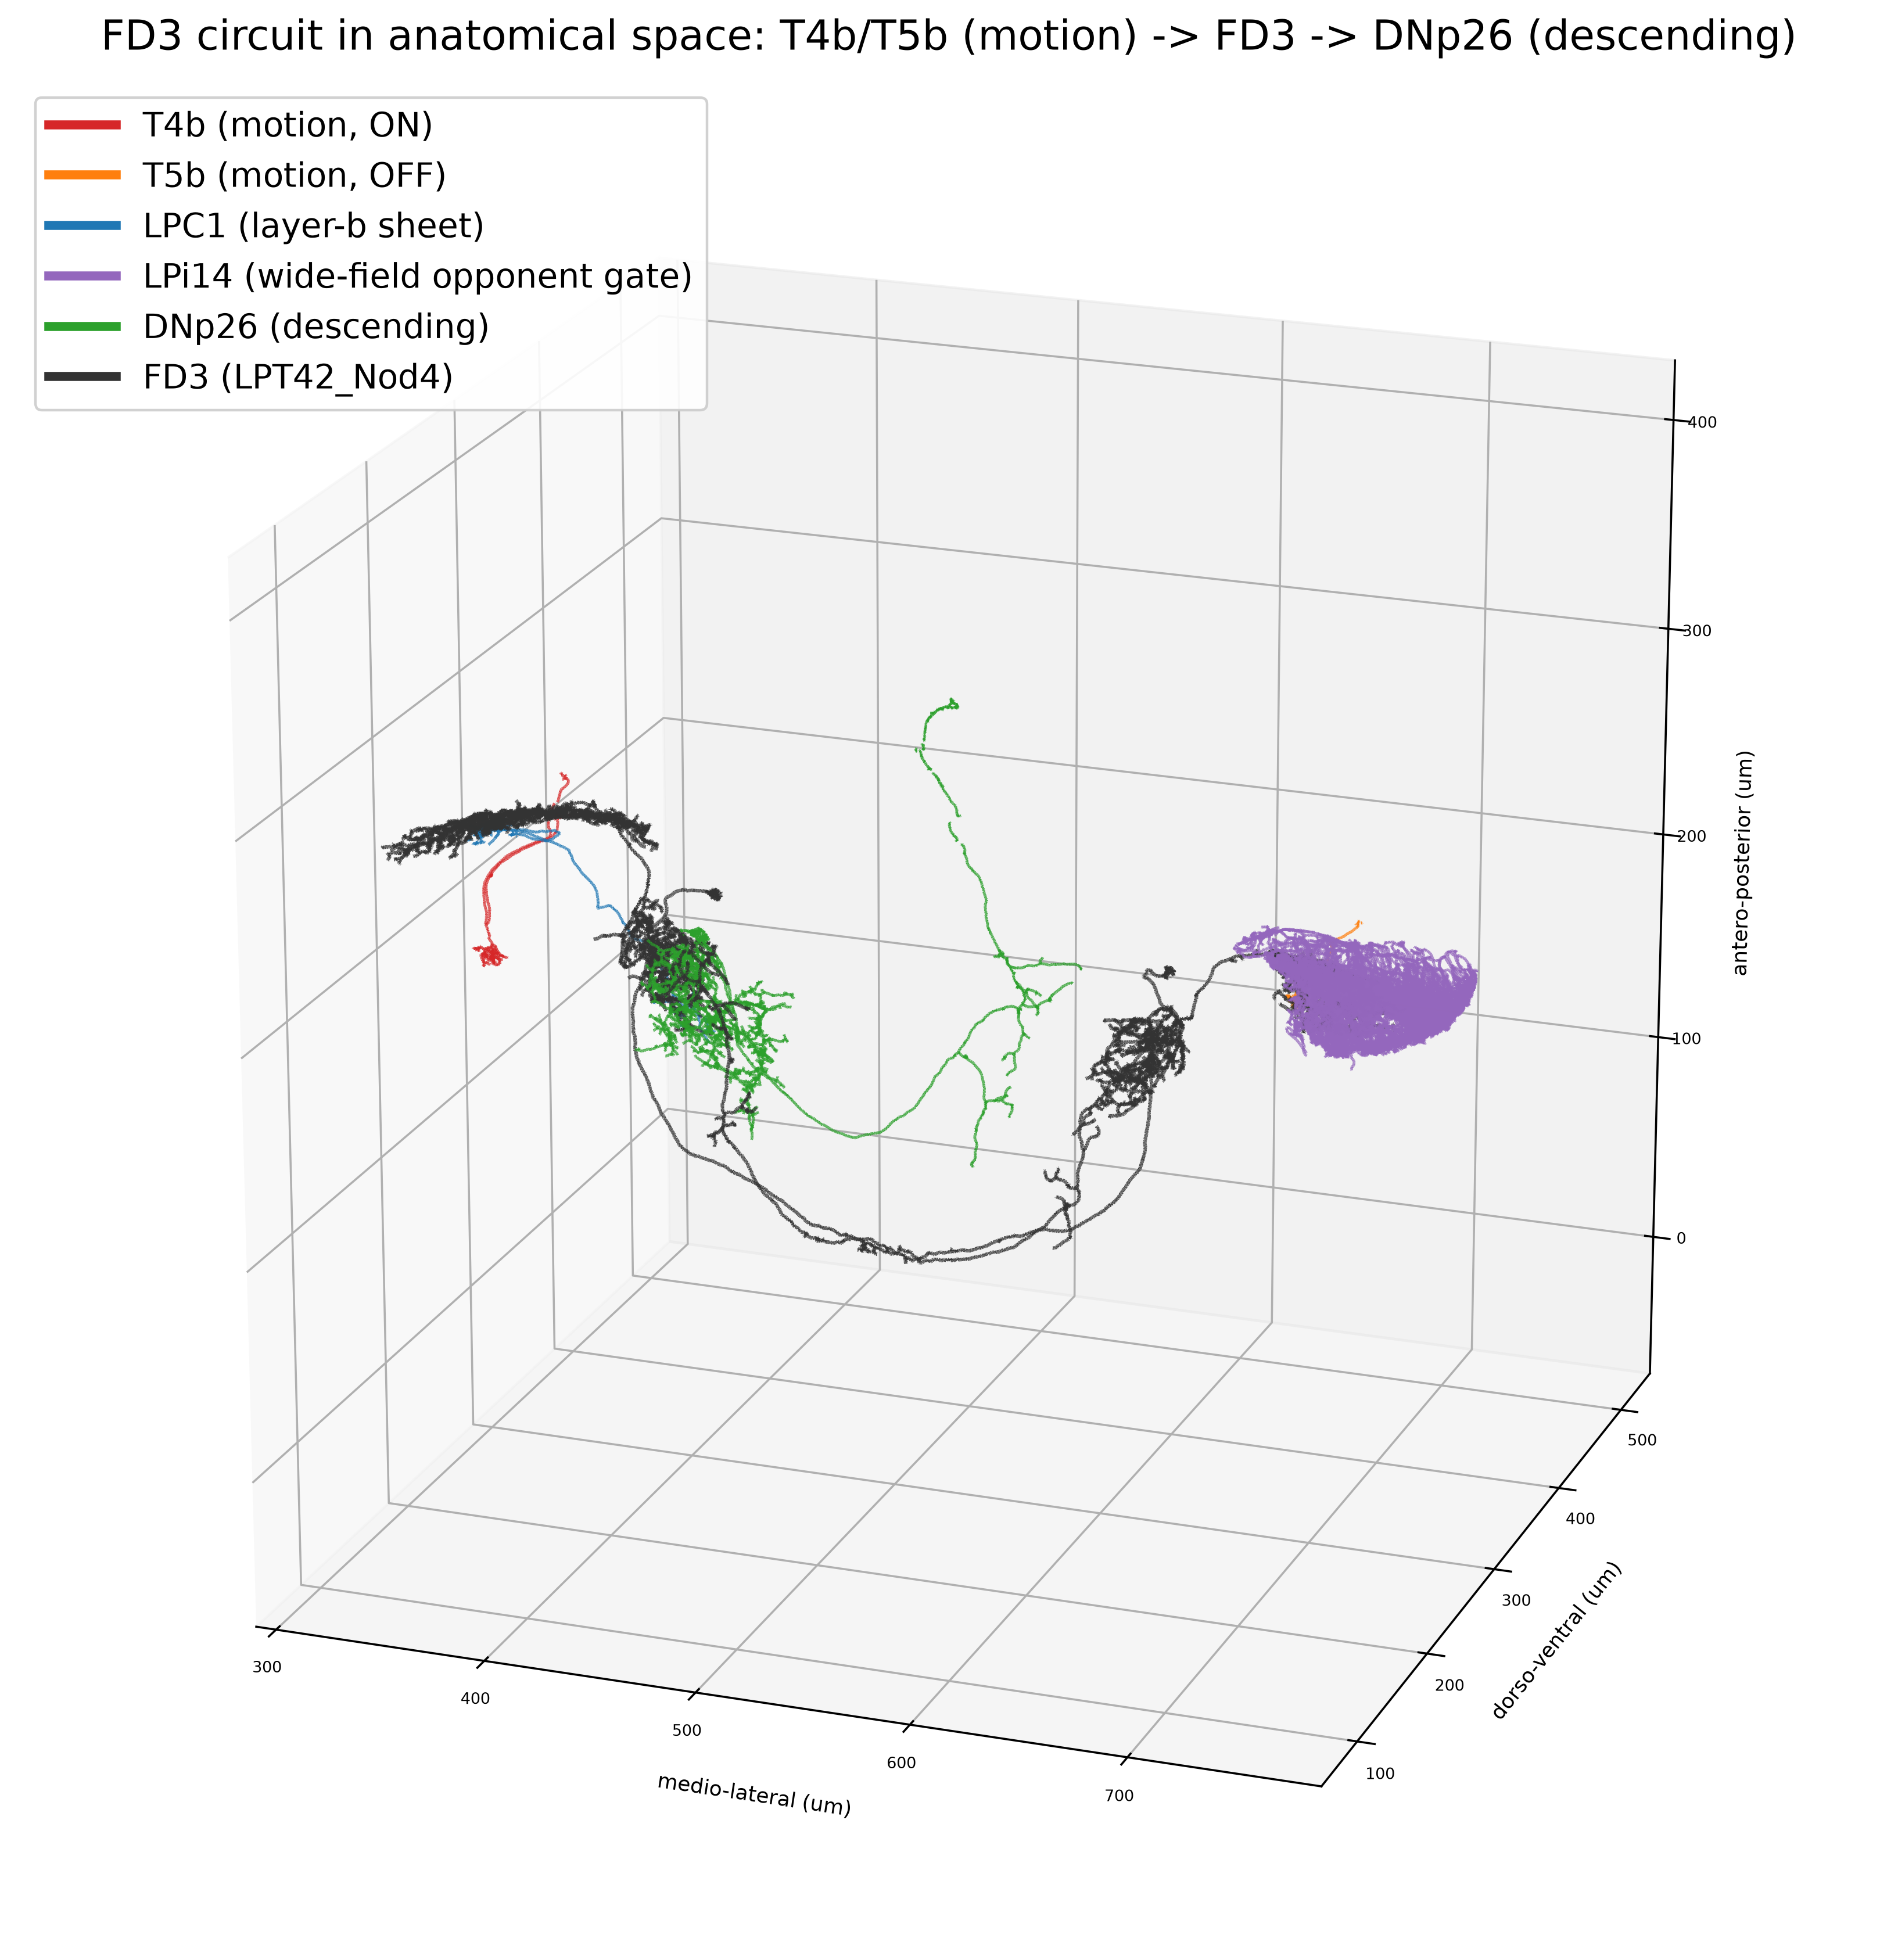
\includegraphics[width=\textwidth,height=0.86\textheight,keepaspectratio]{figures/fd3_circuit_3d.png}
\caption{\textbf{The circuit in the brain.} Reconstructed neurons of the FD3 pathway in their true anatomical positions: the \ttt{T4b} (ON) and \ttt{T5b} (OFF) motion detectors, both FD3 cells with their axons crossing toward the midline, and the descending neuron \ttt{DNp26}, whose dendrite meets FD3's axon terminal before descending toward the nerve cord.}\label{fig:circuit3d}
\end{figure}


\section{The central cells that converge on FD3}

The motion detectors are only about 25.1\% of FD3's input. The larger share comes from central and optic-lobe projection inputs, led by \ttt{LPC1} (acetylcholine, layer b), \ttt{LLPC3} (acetylcholine, layer d), \ttt{LLPC2} (acetylcholine, layer c), \ttt{LPi14} (gaba, layer a). These inputs are not a single layer-b excitatory copy of the T4/T5 drive: the leading set includes cholinergic, GABAergic and glutamatergic types, and their dominant layer annotations span horizontal and vertical channels. In the current derived table, 1 leading central type is marked as a layer-b carrier. FD3 is therefore built from a back-to-front T4/T5 motion core plus broader contextual and inhibitory inputs. This is a wiring description; the sign and function of each non-T4/T5 partner remain hypotheses unless supported by transmitter identity or physiology.

\section{Inhibition from the other eye}

FD3 is not only excited by an object on its own side; it is also inhibited by wide-field motion, including motion seen by the \emph{opposite} eye. In the connectome FD3 receives input from inhibitory (GABAergic) cells on the far side of the brain, with classified synapses in both the front-to-back and back-to-front channels but dominated by the progressive channel, consistent with Egelhaaf's description of contralateral inhibition. Measured this way, FD3's crossed inhibition is direction-dominant (mostly front-to-back) rather than evenly bidirectional, and it is the \emph{opposite} dominant direction from the FD1 cell's crossed inhibition -- a genuine contrast, though the fine split of the minority channel is below what the current annotation can resolve. The report therefore treats the crossed inhibitory motif as present and compatible with physiology rather than as a fully enumerated mechanism. Its computational role remains a hypothesis: crossed inhibition is positioned to suppress wide-field background motion, but the connectome alone does not measure the resulting membrane-potential response.

\section{FD3 is a parallel arm, not a copy of FD1}

Putting the input side together with the identity and output reports, FD3 emerges as a candidate sensory-to-descending channel that runs in parallel to the FD1 arm and is tuned to the opposite direction. Both cells end on the same steering neuron, \ttt{DNp26}, but they are driven differently: FD1 reads front-to-back motion through a centrifugally gated sheet, whereas FD3 reads back-to-front motion, pooled from both ON and OFF detectors and a broad set of columnar sheets, with no such gate and with crossed inhibition from the other eye. The connectome thus supports a model in which oppositely tuned figure-sensitive arms converge on overlapping descending steering targets. Whether this anatomical convergence implements direction-invariant figure tracking requires physiology or perturbation.

\section{What the data can and cannot settle}

\textbf{Motion is a fraction of the input.} The statement that FD3's motion drive is almost entirely back-to-front refers to its \ttt{T4}/\ttt{T5} input specifically; that motion input is itself only about a quarter of FD3's total input, and both numbers are reported so the first is not mistaken for the second. \textbf{The upstream cascade is general wiring.} The photoreceptor-to-detector cascade is measured cell-type by cell-type across the optic lobe and matches the known column wiring; it is shown as the pathway that culminates in FD3's detectors, not as a per-object trace unique to FD3. \textbf{The ON/OFF and transmitter labels are from physiology.} That \ttt{T4} is the ON and \ttt{T5} the OFF detector, and that the photoreceptors are histaminergic, come from published physiology; the connectome supplies the connections and the cell names, not the sign of each cell \cite{maisak2013,hardie1989}. (The automated transmitter table mislabels the photoreceptors, and that value is not used.) \textbf{The crossed inhibition is only partly resolved.} The inhibitory partners from the opposite eye are sparse in the current annotation, so the bidirectional inhibition is reported as present and consistent with the physiology rather than fully enumerated. \textbf{FD3 is two cells.} As in the other reports, FD3 is a single left/right pair, so the result rests on the two cells agreeing and on the thousands of synapses each receives, not on a population average.

\section{Methods and provenance}

\textbf{Connectome.} Inputs are read from the FlyWire FAFB brain connectome (materialization v783) on the \ttt{offline} track. \textbf{Direct inputs}: presynaptic partners of \ttt{LPT42\_Nod4}, aggregated by type and split into motion detectors (with their lobula-plate layer composition), columnar projection sheets, and inhibitory cells, with contralateral input identified by soma side. \textbf{Upstream cascade}: the presynaptic \ttt{T4b}/\ttt{T5b} cells that drive FD3 are followed one step back to their medulla inputs, and the lamina and photoreceptor layers are confirmed present. \textbf{Crossed inhibition}: contralateral GABAergic partners stratified by the lobula-plate layer their type reads. \textbf{Figures}: neuron shapes are reconstructed skeletons; synapse positions are the real synaptic coordinates; the eye-coordinate map uses each detector's retinotopic column. \textbf{Reproducibility}: built from the Family-P verification JSON by the FD3 report CLI. Primary track: \ttt{offline}.

\clearpage\part{Outputs: descending and motor-system partners}

\textbf{Summary.}\quad The figure-detection cell FD3 -- the cell type \ttt{LPT42\_Nod4} in the fly connectome -- is anatomically positioned to report a small moving object in the visual field. For that signal to influence movement it must reach \emph{descending neurons}: cells that project from brain circuits into the ventral nerve cord and contact motor-control networks. This report follows FD3's output to those neurons. We find that FD3 contacts about 24 descending neurons directly, and that its single strongest direct target is \ttt{DNp26} -- the very same wing-steering command neuron on which the previously mapped FD1 analysis converges, so the two figure-cell arms share a major descending target. Beyond this direct route, FD3 reaches a much larger set of descending neurons through one relay step via its strongest central partners. Following every identified descending neuron into the male nerve-cord connectome, where each is matched to the muscles it drives, shows that FD3's descending output is directed most strongly toward the \emph{wing-steering} motor system in this anatomical proxy, with the principal target steering the \emph{opposite} wing. This supports a testable steering hypothesis rather than proving a behavioral command.

\section{Introduction}

\textbf{From a figure signal to a movement.}\quad
A figure-detection cell that fires when a small object moves is only useful to the animal if its
signal can reach the muscles. In the fly, every motor command leaves the brain through a
numerically small population of \emph{descending neurons} (DNs), each of which projects from the
brain into the ventral nerve cord and there contacts motor-control networks~\cite{namiki2018}.
Identifying which descending neurons a visual cell drives, and which muscles those neurons in turn
contact, therefore converts an anatomical identity into a concrete behavioural hypothesis.

\textbf{The template: the FD1 steering arm.}\quad
The figure-ground circuit this work belongs to has already been traced on its FD1 branch in the
companion analysis. There,
the figure signal carried by the cell type \ttt{Nod1} reaches the descending neuron \ttt{DNp26}, a
convergent wing-steering command neuron, and \ttt{DNp26} drives contralateral wing-steering muscles
(\ttt{hg1}, \ttt{i1}, \ttt{hg2}). The question here is whether FD3 -- a regressive,
fronto-lateral figure cell distinct from FD1 -- feeds the same kind of motor pathway, and if so
through which neurons.

\textbf{What we measure.}\quad
We follow FD3's output along two routes. The \emph{direct} route is the set of descending neurons
that receive synapses straight from FD3's axon. The \emph{relayed} route is the set reached one
synapse further on, through FD3's strongest central (non-descending) partners. For every descending
neuron found on either route we then cross into the male whole--central-nervous-system connectome,
which -- unlike the brain-only dataset -- includes the nerve cord, and read off the motor neurons,
muscles and wing side each descending neuron contacts. Egelhaaf, in the third part of his 1985
study, argued that the FD cells serve figure-tracking and the fixation of a moving object; the motor
read-out here is an anatomical counterpart of that behavioural proposal~\cite{egelhaaf1985c}.

\section{The descending neurons FD3 contacts directly}

FD3 makes 138 output synapses onto 24 descending neurons. The leading targets are \ttt{DNp26}, \ttt{DNp12}, \ttt{DNg82}, \ttt{DNge094}, \ttt{DNa07}, \ttt{DNp31} (Fig.~\ref{fig:dnrank}). The single strongest is \ttt{DNp26}; about 58.0\% of FD3's direct descending output goes to neurons already known to drive wing-steering muscles. Both FD3 cells -- one per side of the brain -- contribute (right cell: 74 synapses; left cell: 64 synapses), so the projection is bilateral, as the cell is.

\ttt{DNp26} is notable: it is the same convergent wing-steering command neuron that the FD1 cell reaches through \ttt{Nod1}. FD3 and FD1, two figure cells tuned to opposite directions of motion and different parts of the visual field, therefore converge on a shared descending target. This is anatomical support for a common figure-tracking output stage.

\begin{figure}[H]\centering
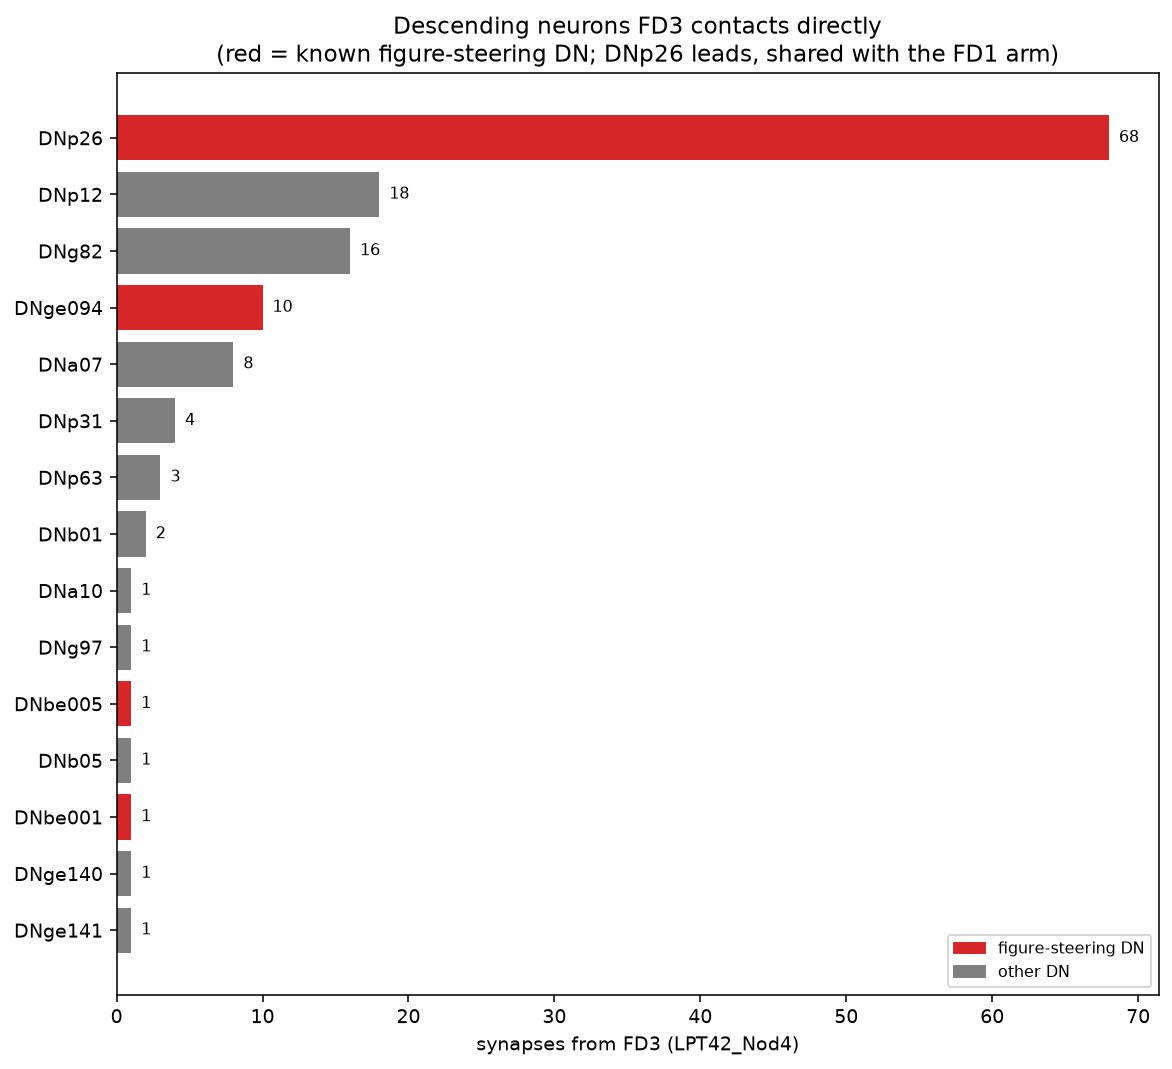
\includegraphics[width=\textwidth]{figures/fd3_dn_ranking.png}
\caption{\textbf{The descending neurons FD3 contacts directly.} Each bar is one descending-neuron type, ranked by the number of synapses it receives from FD3. Red marks neurons already known to drive wing-steering muscles. \ttt{DNp26}, the figure-steering command neuron shared with the FD1 arm, leads.}\label{fig:dnrank}
\end{figure}


\section{The descending neurons FD3 reaches through a relay}

Beyond the neurons it drives directly, FD3 sends most of its output to central brain neurons rather than to descending neurons. Taking FD3's strongest such partners (those receiving at least 30 synapses from FD3 -- 16 cell types, led by \ttt{PLP230}, \ttt{WED075}, \ttt{PLP178}, \ttt{PLP012}, \ttt{PLP078}, \ttt{PS010}) and following \emph{their} output reaches a further 263 descending neurons (Fig.~\ref{fig:dnchannels}). This relayed route is broad where the direct route is focused: it spreads onto many more descending neurons, the larger of the two routes by total synapses.

Crucially the two routes are not unrelated. 16 descending-neuron types are reached \emph{both} directly and through the relay, including \ttt{DNa10}, \ttt{DNb01}, \ttt{DNb05}, \ttt{DNbe001}, \ttt{DNbe005}, \ttt{DNg82}, \ttt{DNg97}, \ttt{DNge094}. These overlaps show that the relay reaches some of the same DN classes as the direct route. Because the size of the relayed set depends on how strong a partner has to be to count, we report that sensitivity explicitly (Fig.~\ref{fig:dnchannels}b): the count grows smoothly as the threshold is relaxed.

\begin{figure}[H]\centering
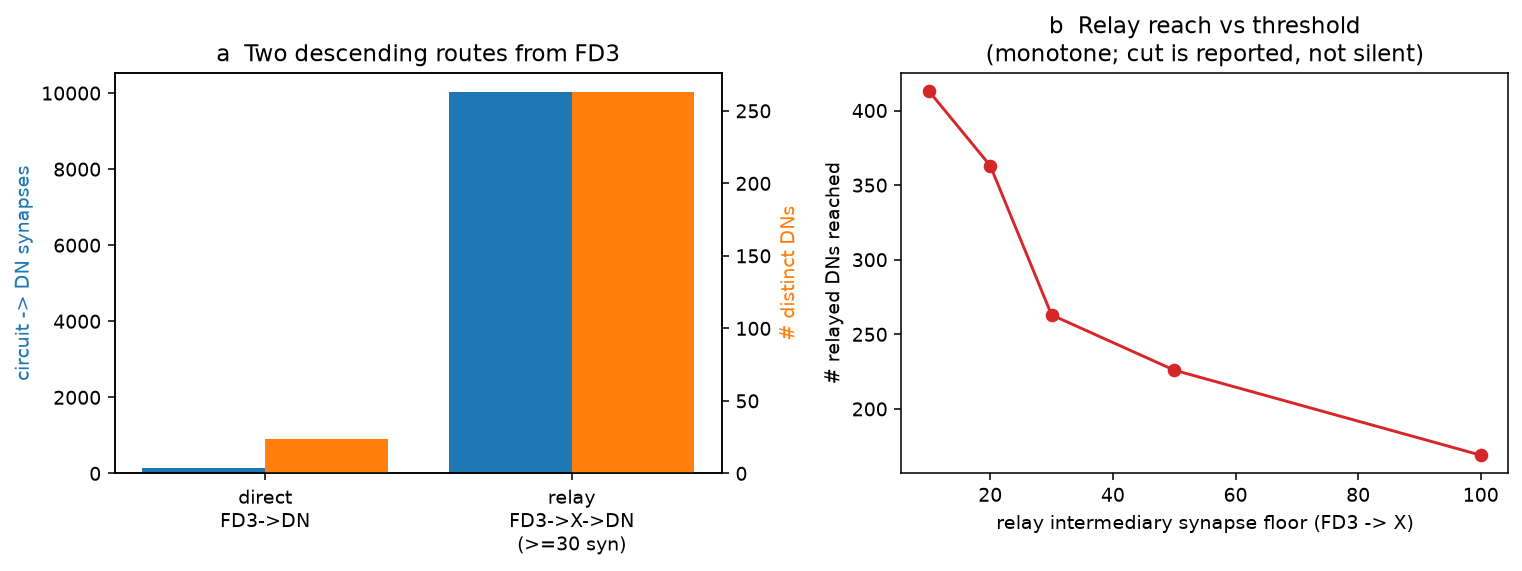
\includegraphics[width=\textwidth]{figures/fd3_descending_channels.png}
\caption{\textbf{Two descending routes from FD3.} (a) The direct route (FD3 $\rightarrow$ descending neuron) is focused; the relayed route (FD3 $\rightarrow$ central partner $\rightarrow$ descending neuron) is broader, reaching many more neurons. (b) The number of relayed descending neurons as the partner-strength threshold is varied -- it changes smoothly, so the result does not hinge on one cut-off.}\label{fig:dnchannels}
\end{figure}


\section{Motor systems contacted by those neurons}

Each descending neuron FD3 reaches can be matched, by its standard name, to a cell in the male nerve-cord connectome and from there to the motor neurons and muscles it contacts. Weighting every neuron by how strongly FD3 drives it, the largest share of FD3's descending output -- 43.5\% -- reaches the \emph{wing-steering} muscles (Fig.~\ref{fig:motorsys}). Smaller shares reach the neck (gaze), abdominal and haltere systems. This anatomical weighting supports a steering hypothesis, but it does not by itself prove that FD3 activity drives steering behavior.

The principal target, \ttt{DNp26}, drives the \emph{contralateral} wing (its wing-steering output goes overwhelmingly to the side opposite its own cell body) through the steering muscles \ttt{hg1}, \ttt{hg2}, \ttt{i1}, matching from FD3's vantage point the same muscle targets found on the FD1 arm. A figure seen to one side thus acts, through FD3 and \ttt{DNp26}, on a pathway with the laterality needed for asymmetric wing steering.

\begin{figure}[H]\centering
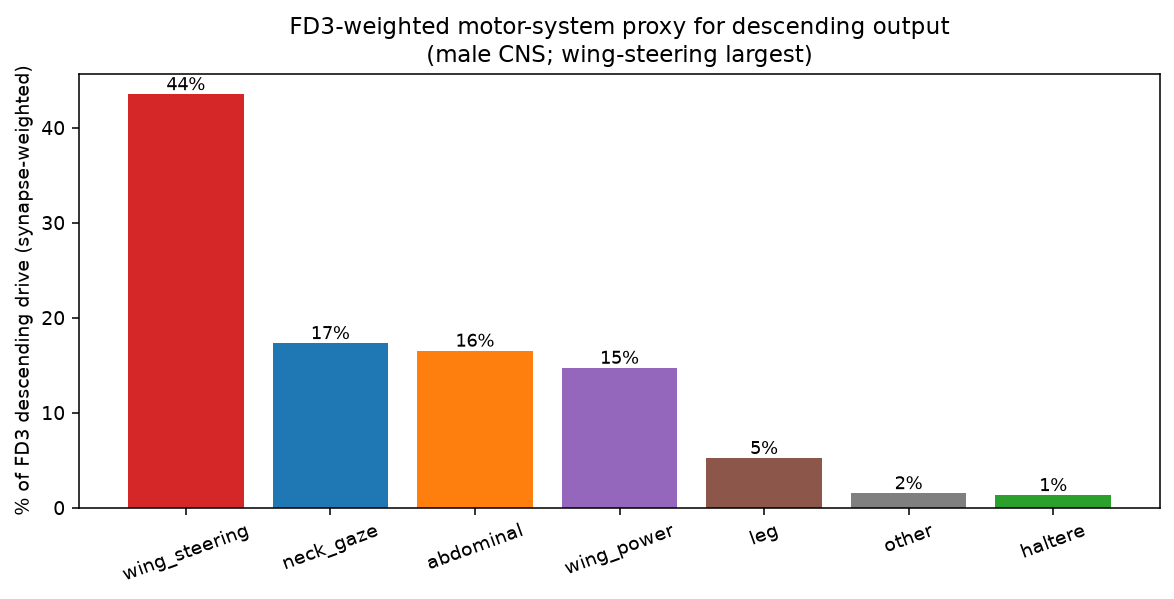
\includegraphics[width=\textwidth]{figures/fd3_motor_systems.png}
\caption{\textbf{Motor-system proxy.} The motor systems reached by FD3's descending output, weighted by how strongly FD3 drives each descending neuron. Wing-steering has the largest FD3-weighted share.}\label{fig:motorsys}
\end{figure}


\begin{figure}[H]\centering
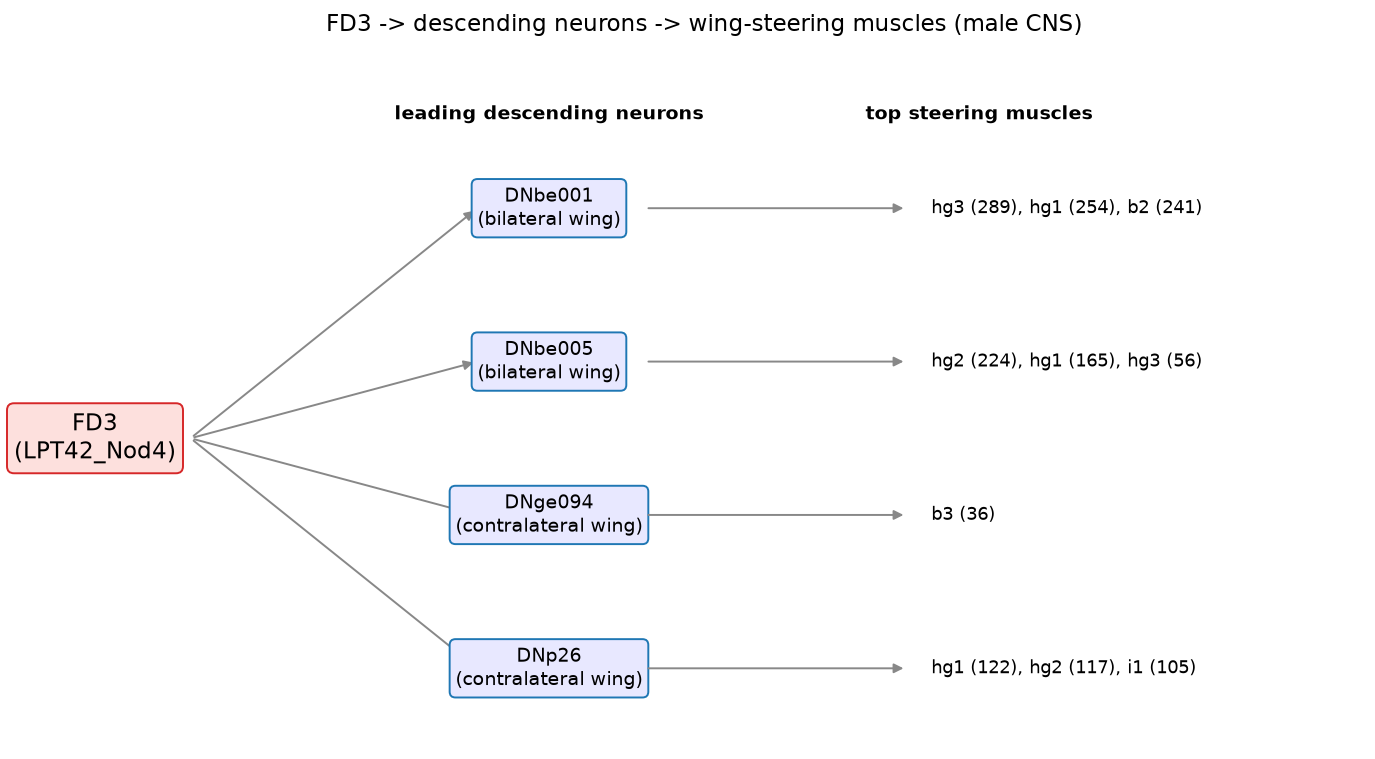
\includegraphics[width=\textwidth]{figures/fd3_brain_to_muscle.png}
\caption{\textbf{From FD3 to the wing muscles.} The leading wing-steering descending neurons FD3 reaches, the wing each one steers, and the steering muscles it drives in the nerve cord.}\label{fig:b2m}
\end{figure}


\section{Functional implications}

Three anatomical facts make FD3 a concrete candidate pathway for figure-directed steering. First, FD3 reaches descending neurons directly and through one relay step, with the FD3-weighted motor proxy largest for wing steering. Second, FD3 and the FD1 arm share \ttt{DNp26}, so figure signals with different preferred directions converge on at least one major descending target. Third, \ttt{DNp26} contacts the contralateral wing-steering muscles in the male CNS map. These results specify a testable sensorimotor hypothesis: FD3 activity should bias wing-steering output for laterally seen regressive figures. Proving that hypothesis requires physiology or perturbation.

\section{What the data can and cannot settle}

\textbf{The exact counts are track-specific.} The synapse and DN counts are reported for the primary verification track named in Methods. If a live or alternate-release rerun is used later, those absolute counts should be reported separately rather than silently merged. \textbf{The relay set depends on a threshold.} The direct descending targets are unambiguous -- they are the neurons FD3 synapses onto. The relayed set depends on how strong a central partner must be to be followed; we report the full sensitivity of the count to that choice rather than fixing a single number. \textbf{The muscle map crosses two connectomes.} The muscles each descending neuron drives are read from a second, male nerve-cord connectome, and the link between the two datasets is the shared neuron name. Where a descending neuron carries the same name in both, the match is direct; a neuron without a named nerve-cord counterpart simply contributes no muscle information and is not forced into one. \textbf{FD3 is two cells.} As in the identity report, FD3 is a single left/right pair, so the result rests on the two cells agreeing and on the thousands of synapses each makes, not on a population average.

\section{Methods and provenance}

\textbf{Connectomes.} The descending targets are read from the FlyWire FAFB brain connectome (materialization v783); a neuron counts as descending by its \ttt{super\_class} annotation. The motor read-out is the male whole-CNS connectome (male-cns:v1.0), reached offline; descending neurons are matched between the two by their shared Janelia name. \textbf{Direct route}: postsynaptic partners of \ttt{LPT42\_Nod4} whose super-class is descending, aggregated by type. \textbf{Relayed route}: FD3's strongest non-descending partners (above a reported synapse floor) and their descending output, attributed to the intermediary type, with the count's threshold-sensitivity reported. \textbf{Motor systems}: each descending neuron's male-CNS motor output classified by motor-neuron subclass (wing-steering, wing-power, neck/gaze, haltere, leg, abdominal); wing laterality is the descending neuron's soma side versus the motor neuron's. \textbf{Reproducibility}: built from the Family-L verification JSON by the FD3 report CLI. Primary track: \ttt{offline}.

\clearpage\part{The functional figure-ground circuit within FD3}

\textbf{Summary.}\quad The figure-detection cell FD3 (\ttt{LPT42\_Nod4}) sits inside a large web of connections -- thousands of partners in and out. This report first maps that web comprehensively, then picks out the working figure-ground circuit within it and names every element, in the same terms as the previously described FD1 pathway. We find that the motion signal reaches FD3 through a named intermediate sheet -- the cell type \ttt{LPC1}, the one neighbouring sheet that reads the same back-to-front motion channel FD3 does -- so the pathway is \ttt{T4b}/\ttt{T5b} $\rightarrow$ \ttt{LPC1} $\rightarrow$ FD3, with the sibling sheets adding a four-direction motion-context surround. And we find that FD3 is shaped by \emph{two} complementary wide-field inhibitory gates. \ttt{LPi14} plays the role the wide-field cell VCH plays for FD1 -- it pools motion across the field, feeds back onto the detectors, gates the sheet, and inhibits FD3 -- but is a different cell class, tuned to the opposite direction, so it is an \emph{opponent} gate. \ttt{LPi12} is the \emph{same-direction} surround Egelhaaf predicted: a regressive wide-field cell that acts one stage upstream, dominating the inhibition of FD3's own \ttt{T4b}/\ttt{T5b} detectors while touching FD3 only weakly. The two gates are complementary, not competing: \ttt{LPi12} does not replace \ttt{LPi14}.

\section{FD3's connectivity, comprehensively}

Before isolating the figure-ground circuit we map FD3's whole connectivity. FD3 receives about 13157 input synapses from roughly 2991 partner cells, and makes about 15122 output synapses onto roughly 8435 partners. The inputs are dominated by the motion detectors and a handful of neighbouring columnar sheets together with inhibitory cells; the outputs are broadcast widely to central brain cells and, through the descending neurons, to the steering muscles. Against this backdrop the working figure-ground circuit is a small, identifiable subset, highlighted below.

\begin{figure}[H]\centering
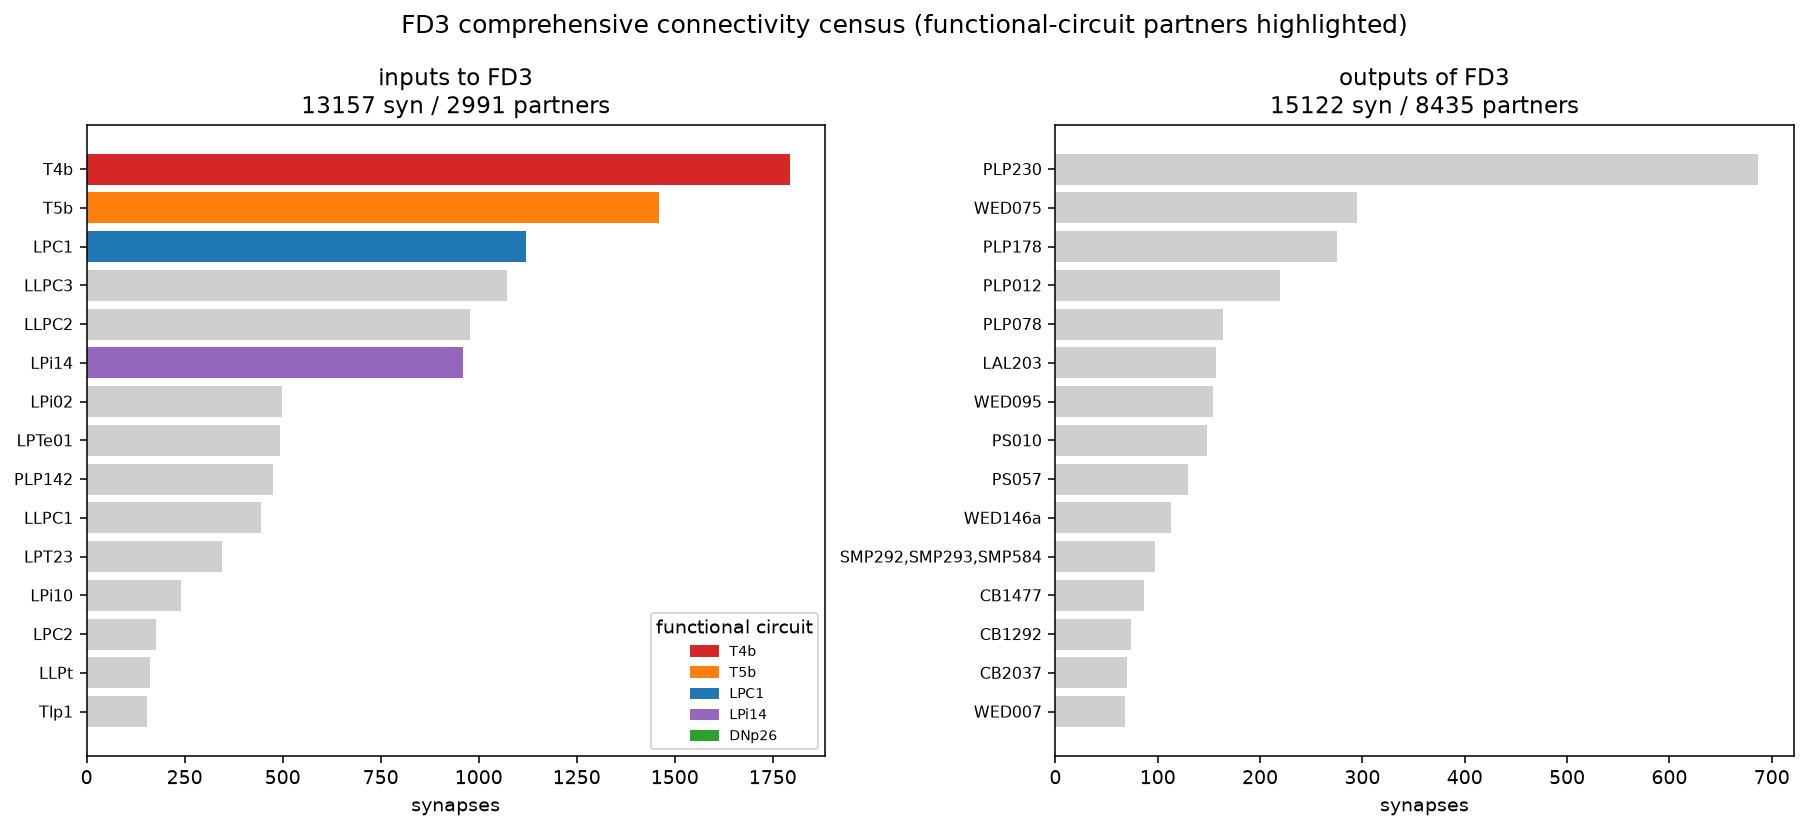
\includegraphics[width=\textwidth]{figures/fd3_connectivity_wheel.png}
\caption{\textbf{FD3's comprehensive connectivity.} Every major input (left) and output (right) partner type of FD3. The cells of the functional figure-ground circuit are drawn in colour; the rest of the web is greyed, so the circuit stands out from the full connectivity.}\label{fig:wheel}
\end{figure}


The inputs also land in a structured way on the cell. Splitting FD3's input synapses between its dendrite and its axon shows that essentially all of the input -- the motion drive, the sheet, and the inhibition alike -- arrives on the dendritic arbour in the lobula plate, while the axon carries the cell's output across the midline. FD3 is thus a cleanly polarised neuron, and the inhibition is applied on the same arbour that receives the excitation.

\begin{figure}[H]\centering
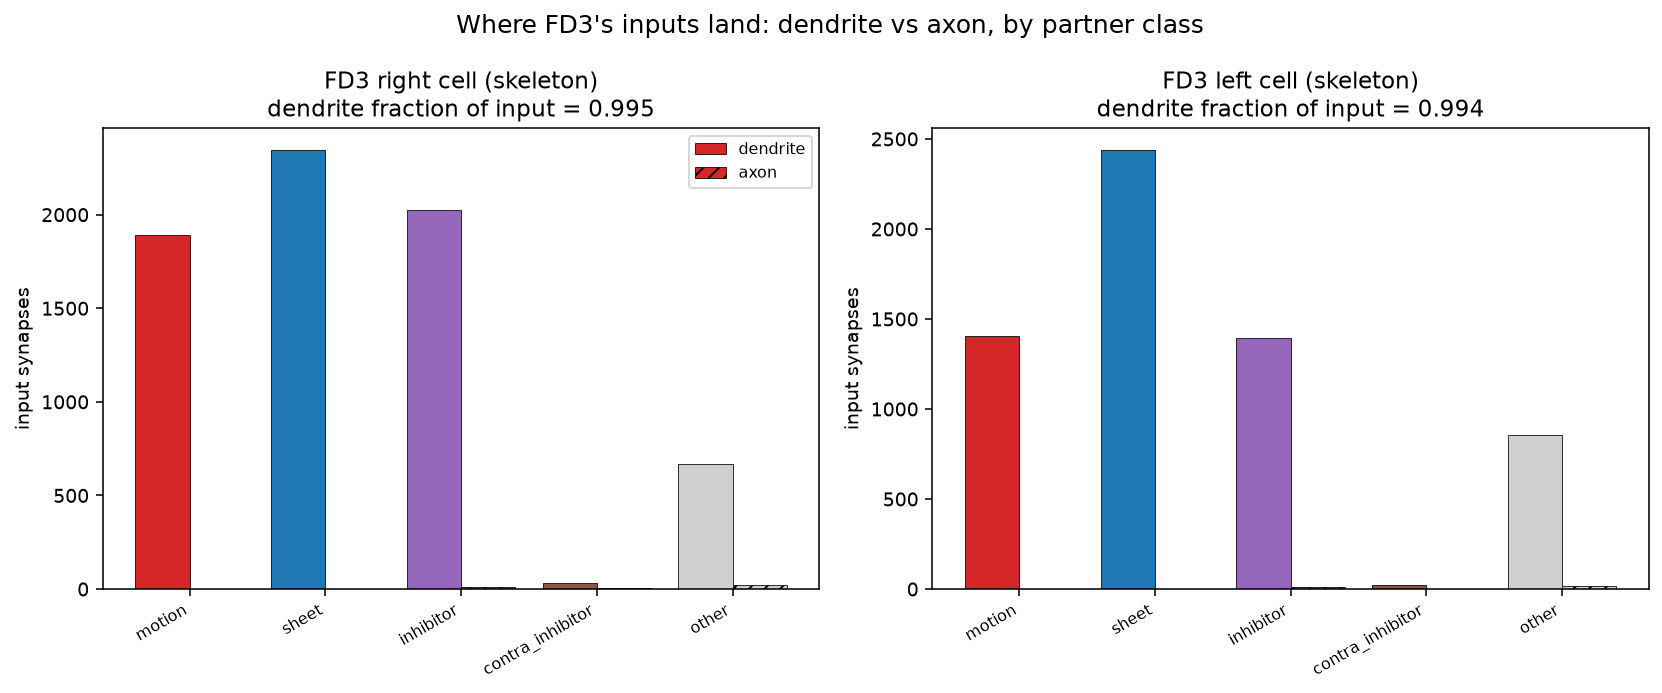
\includegraphics[width=\textwidth]{figures/fd3_compartment_split.png}
\caption{\textbf{Where inputs land.} Input synapses to each FD3 cell, split between the dendrite and the axon and coloured by the class of partner. Almost all input -- excitatory and inhibitory -- is on the dendrite.}\label{fig:compartment}
\end{figure}


\section{Naming the sheet: T4b/T5b $\rightarrow$ LPC1 $\rightarrow$ FD3}

For the FD1 cell, the motion detectors do not contact the figure cell directly; they first drive a retinotopic sheet of cells (\ttt{LLPC1}) that then relays to FD1. FD3 has the same architecture, and the sheet that fills the equivalent slot is \ttt{LPC1}. Of the neighbouring sheets that contact FD3, \ttt{LPC1} is the only one that reads the same back-to-front (layer-b) motion channel FD3 is tuned to (its sibling sheets read the vertical up/down channels instead), it is cholinergic (excitatory), and it is driven by the very same \ttt{T4b}/\ttt{T5b} detectors (1120 synapses onto FD3). It is also genuinely retinotopic: the detectors feeding each \ttt{LPC1} cell come from a tight local patch of the eye, far tighter than chance, so it preserves the spatial map rather than pooling globally.

So the intermediate is best described as a small \emph{set} of sibling sheets (LPC1, LLPC3, LLPC2, LPC2) of which \ttt{LPC1} is the direction-matched, horizontal member carrying the figure signal. Notably, FD1's own sheet (\ttt{LLPC1}) is \emph{not} a major input to FD3 -- FD3 reads a different sheet, as befits its opposite direction preference.

The sibling sheets are not simply ``vertical context'': each reads its own cardinal motion channel, so FD3's sheet-relayed input spans all four directions. Rolling the sheets' synapses onto FD3 up by the motion channel each one reads gives \ttt{LPC1} (back-to-front, FD3's own direction) 29.5\%, \ttt{LLPC3} (downward) 28.2\%, \ttt{LLPC2}/\ttt{LPC2} (upward) 30.5\%, and \ttt{LLPC1} (front-to-back, the opposite direction) 11.8\% of the sheet input. The direction-matched channel is thus a \emph{minority} (29.5\%) of what the sheets deliver: FD3 reads its own regressive channel through \ttt{LPC1} plus a near-balanced up/down/opposite \emph{motion-context surround} through the siblings. This is a statement about the \emph{sheet-relayed} input; FD3's \emph{direct} \ttt{T4}/\ttt{T5} drive stays $\sim$99\% back-to-front (Part~II).

\begin{figure}[H]\centering
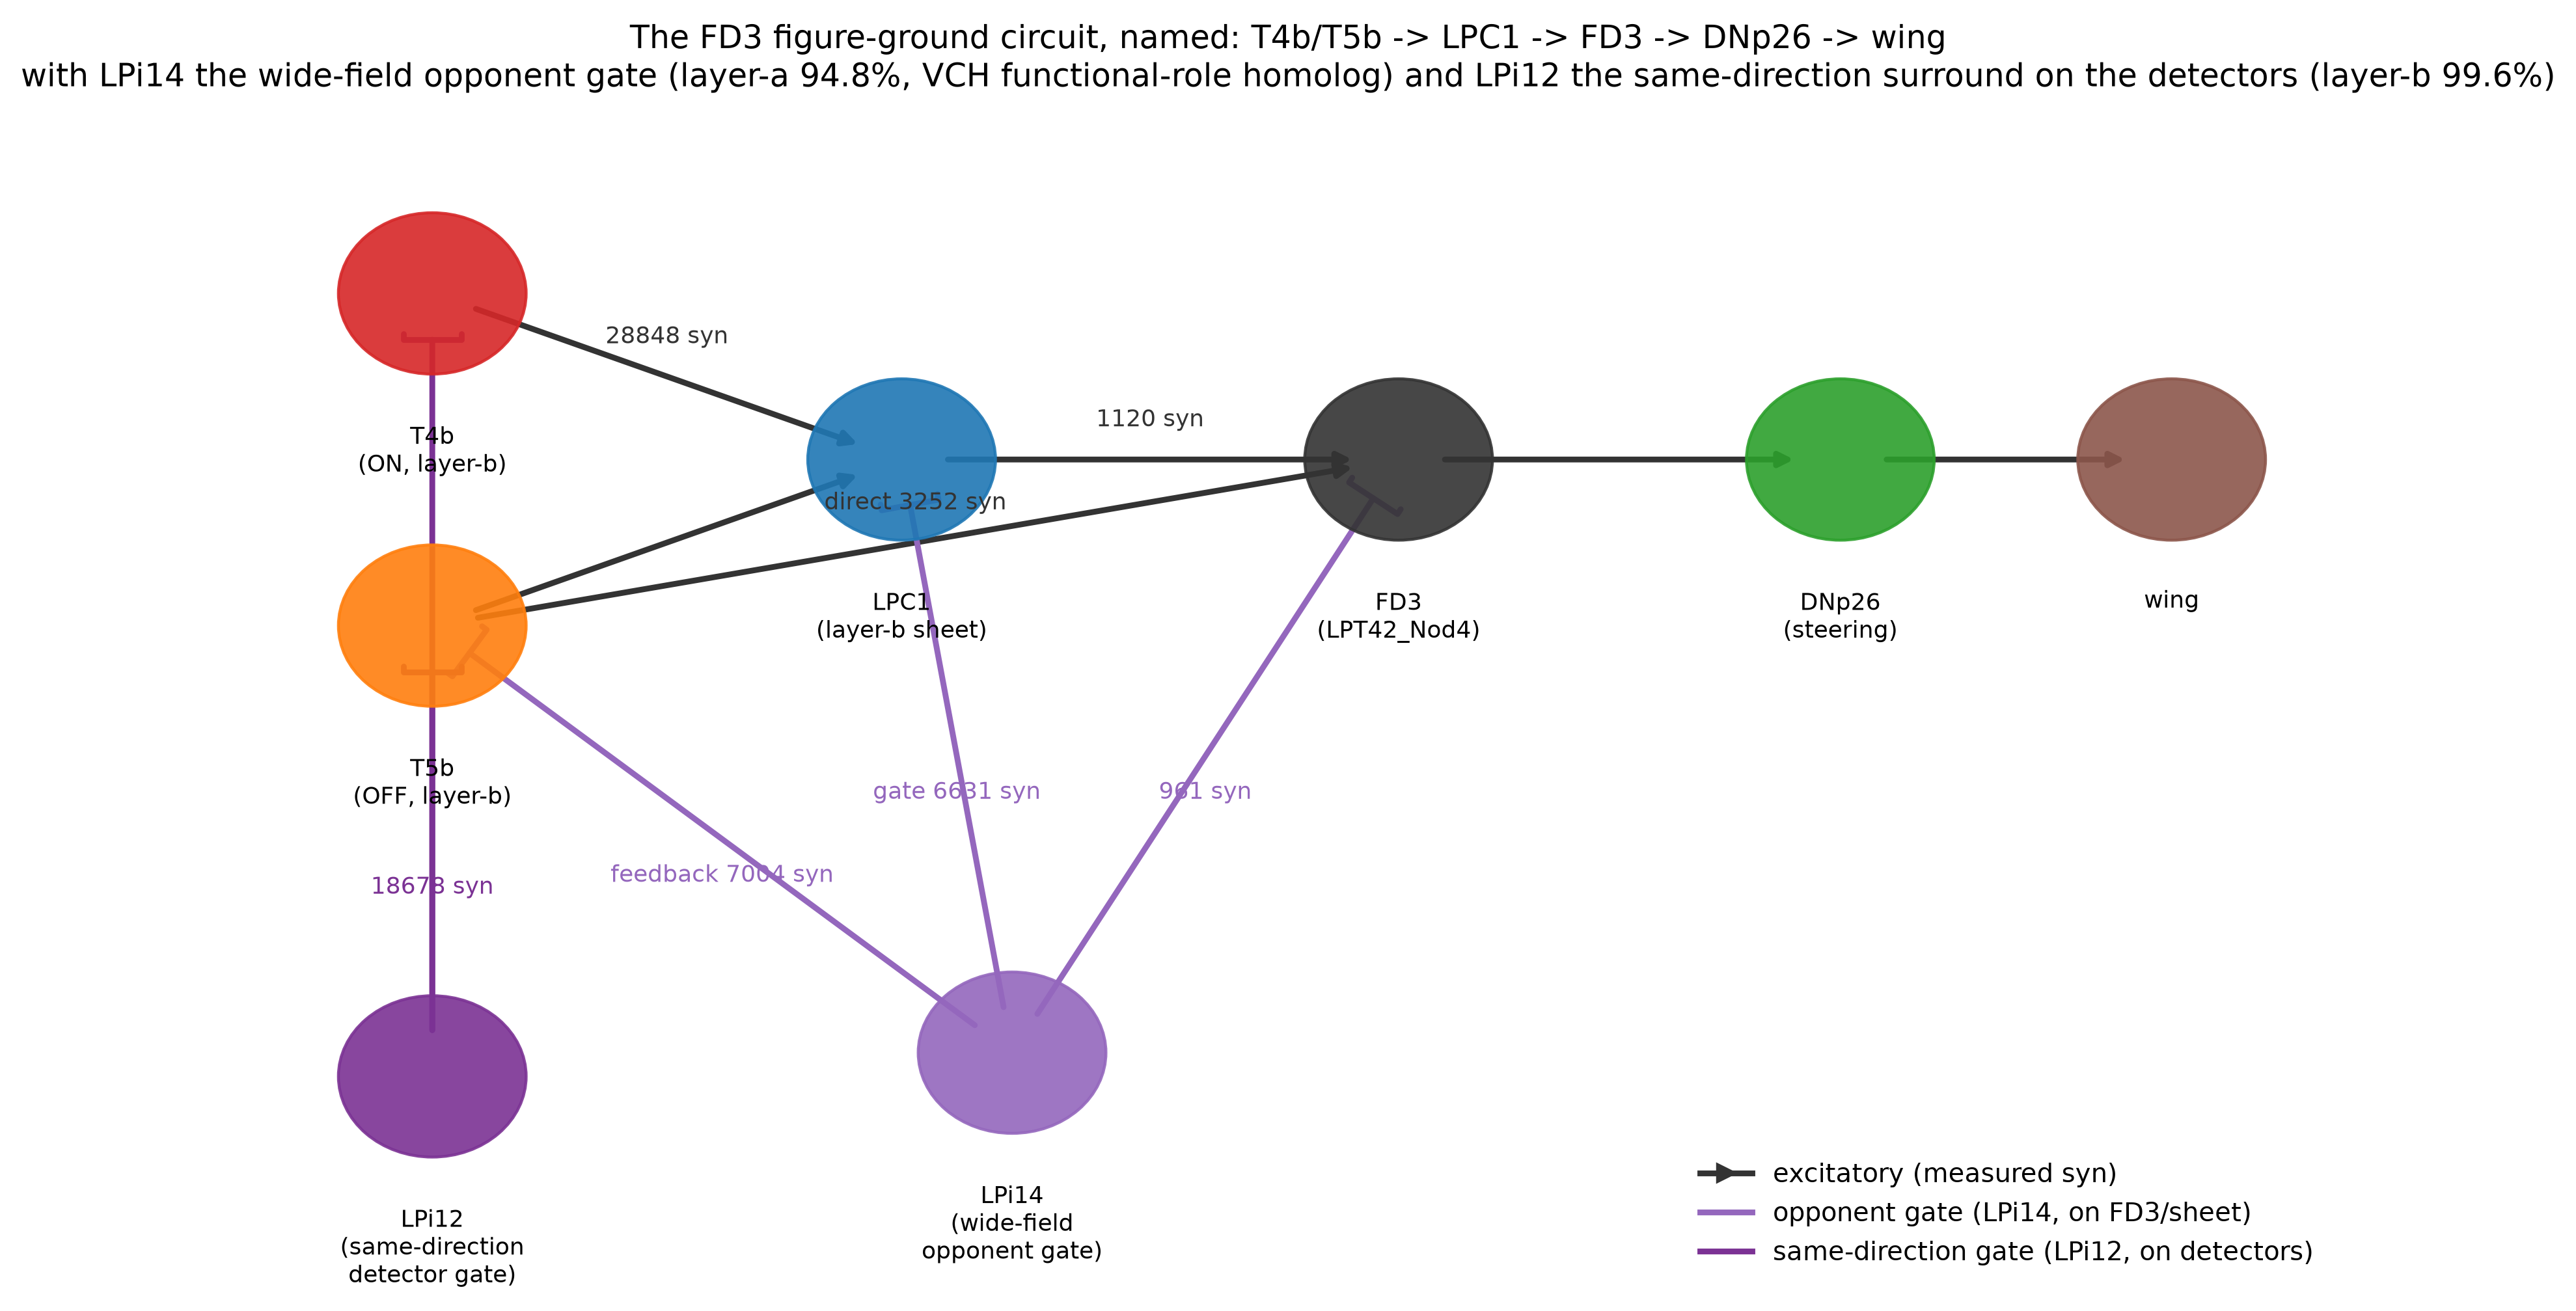
\includegraphics[width=\textwidth]{figures/fd3_functional_circuit_schematic.png}
\caption{\textbf{The named figure-ground circuit, with its two gates.} \ttt{T4b}/\ttt{T5b} motion detectors drive the layer-b sheet \ttt{LPC1}, which relays to FD3; FD3 drives the steering neuron \ttt{DNp26} and the wing. Two wide-field inhibitory cells (flat-headed arrows) gate the circuit at different nodes: the opponent cell \ttt{LPi14} gates the sheet, feeds back onto the detectors, and inhibits FD3; the same-direction cell \ttt{LPi12} pours inhibition onto the \ttt{T4b}/\ttt{T5b} detectors. Numbers are measured synapse counts.}\label{fig:funcircuit}
\end{figure}


\section{Two wide-field gates: an opponent gate and a same-direction surround}

For FD1, a single wide-field cell, VCH, does four things: it pools motion across the whole visual field, feeds that back onto the motion detectors, gates the sheet, and so shapes the figure cell's selectivity. For FD3, the cell that fills that role at the figure-cell and sheet level is \ttt{LPi14}. It pools wide-field motion (72.6\% of its own input is motion detectors), it feeds back onto FD3's \ttt{T4b}/\ttt{T5b} detectors (7004 synapses), it gates the \ttt{LPC1} sheet (6631 synapses), and it inhibits FD3 directly (961 synapses -- 35.94\% of all the inhibition FD3 receives). In wiring terms it stands where VCH stands for FD1.

There are three honest differences from VCH, and they matter. First, \ttt{LPi14} is a lobula-plate \emph{intrinsic} cell, not a centrifugal cell like VCH -- a different cell class filling the same role. Second, it is tuned to the \emph{opposite} direction from FD3 (it reads front-to-back motion, FD3 reads back-to-front), so it acts as an \emph{opponent} suppressor rather than a same-direction gain control. Third, FD3 does not send much back to it, so the loop is not reciprocal in the way VCH's is. For these reasons we describe \ttt{LPi14} as the \emph{functional} counterpart of VCH -- it plays VCH's part in the circuit -- rather than the same cell type.

Egelhaaf, recording from FD3, inferred a second wide-field inhibitor tuned to the \emph{same} direction as FD3's excitation, to explain how FD3 tells a small object from whole-field motion. Searching the full lobula-plate intrinsic panel resolves it: \ttt{LPi12}, a GABAergic cell tuned to the \emph{same} back-to-front direction as FD3 (99.6\% layer-b). But \ttt{LPi12} does its work at a \emph{different node}: it pours 18678 synapses onto the \ttt{T4b}/\ttt{T5b} detectors themselves -- 43.86\% of its own output, and a larger share of the detectors' total inhibition than \ttt{LPi14} supplies -- while touching FD3 only weakly (68 synapses, 2.54\% of FD3's inhibition) and barely reaching the sheet (165 synapses). So \ttt{LPi12} does \emph{not} replace \ttt{LPi14}; the two are complementary gates at different stages -- an opponent gate on the figure cell and its sheet, and a same-direction surround on the motion detectors.

That \ttt{LPi12} touches FD3 at all is not an accident of its size: its 68 synapses onto FD3 exceed what a size-matched random lobula-plate target would receive from it (null 11.09, $z=2.95$, $p=0.002$), so the (minor) direct contact is a genuine FD3-specific input rather than spillover. Whether either gate produces net suppression, and which carries the effect Egelhaaf measured, is a question for physiology; the connectome supplies the wiring and the direction, not the sign of the response.

\section{The circuit, named end to end}

Putting the pieces together, FD3's figure-ground circuit reads, in full: the \ttt{T4b}/\ttt{T5b} back-to-front motion detectors drive the layer-b sheet \ttt{LPC1} (one of a sibling set that also relays the other three cardinal directions as context), which relays to FD3; FD3 drives the steering command neuron \ttt{DNp26} and thence the wing. Two wide-field gates shape it: the opponent cell \ttt{LPi14} gates the sheet, feeds back onto the detectors, and inhibits FD3 directly; and the same-direction cell \ttt{LPi12} pours inhibition onto FD3's detectors while barely touching FD3 itself. This is the same core architecture as the FD1 arm (detectors $\rightarrow$ sheet $\rightarrow$ figure cell $\rightarrow$ steering command, with wide-field inhibitory gating), built from a different, oppositely-tuned set of cells, and with the same-direction surround Egelhaaf predicted resolved as a distinct detector-level gate. Whether these gates implement the small-versus-wide-field discrimination Egelhaaf described is a functional question the wiring sets up but does not answer.

\section{What the data can and cannot settle}

\textbf{The sheet is a set, and LPC1 is its direction-matched member.} Several sibling sheets contact FD3, carrying all four cardinal motion directions; \ttt{LPC1} is named as the figure-carrying one because it is the only one reading FD3's own (back-to-front) channel, and the multi-direction pooling is reported as sheet-relayed context, not as a change in FD3's own $\sim$99\% back-to-front tuning. \textbf{Two gates, at different nodes, not a replacement.} \ttt{LPi14} is the opponent gate on FD3 and its sheet; \ttt{LPi12} is the same-direction gate on FD3's detectors. The two are named by \emph{where} and \emph{in which direction} they act, normalised against each target's total inhibition so raw synapse counts (and \ttt{LPi14}'s known hub connectivity) do not mislead; \ttt{LPi12} is a minor slice of FD3's own inhibition, so it complements rather than replaces \ttt{LPi14}. \textbf{Sign is not read from wiring.} That a GABAergic contact is inhibitory, and that either gate suppresses FD3's figure response, are expectations from physiology; the connectome supplies the connections and the direction, not the sign or the response. Some inhibitory-looking cells here are predicted glutamatergic, whose sign depends on the receptor and is left open. \textbf{FD3 is one bilateral pair.} As throughout, the result rests on the two cells agreeing (both show the same two-gate asymmetry) and on the thousands of synapses each makes, not on a population average.

\section{Methods and provenance}

\textbf{Connectome.} All connectivity is read from the FlyWire FAFB brain connectome (materialization v783), cross-checked offline. \textbf{Census}: every pre- and postsynaptic partner of \ttt{LPT42\_Nod4}, partitioned by cell class, transmitter, lobula-plate layer and side. \textbf{Sheet}: candidate columnar-projection sheets feeding FD3 scored by their motion-channel tuning, their synapses onto FD3, and a retinotopy test (each sheet cell's detector inputs vs a shuffled-input null). \textbf{Sheet directions}: each sheet's synapses onto FD3 rolled up by the motion channel it reads; a sheet's direction label is used only when its dominant layer beats the runner-up by $\geq$20 percentage points and is stable in $\geq$95\% of synapse resamples. Whether four-direction pooling is FD3-specific is tested against the FD1=Nod1 reference and a random lobula-plate-tangential entropy null. \textbf{Inhibitor}: FD3's inhibitory inputs screened across the full lobula-plate intrinsic panel for wide-field pooling, feedback onto the detectors, gating of the sheet, and direct inhibition of FD3 (the screen does not require a centrifugal cell type). Each candidate's contact is normalised against the target's total inhibition (and the candidate's own output budget) so raw counts and hub connectivity do not mislead; a same-direction candidate's direct-FD3 contact is tested for FD3-specificity against a size-matched random-target permutation null, and every threshold-dependent call is reported across a floor sweep. \textbf{Compartments}: input synapses assigned to the dendrite or axon by nearest point on the reconstructed skeleton. \textbf{Left/right agreement}: FD3 is a bilateral pair, so the two-gate asymmetry and the direction labels are checked on both cells. \textbf{Reproducibility}: rebuilt from the verification JSON. Primary track: \ttt{offline}.

\clearpage

\begin{thebibliography}{11}
\bibitem{egelhaaf1985a} Egelhaaf M. (1985) On the neuronal basis of figure-ground discrimination by relative motion in the visual system of the fly. I. Behavioural constraints imposed on the neuronal network and the role of the optomotor system. \textit{Biological Cybernetics} 52:123--140. doi:10.1007/BF00364003.
\bibitem{egelhaaf1985b} Egelhaaf M. (1985) On the neuronal basis of figure-ground discrimination by relative motion in the visual system of the fly. II. Figure-detection cells, a new class of visual interneurones. \textit{Biological Cybernetics} 52:195--209. doi:10.1007/BF00339948.
\bibitem{egelhaaf1985c} Egelhaaf M. (1985) On the neuronal basis of figure-ground discrimination by relative motion in the visual system of the fly. III. Possible input circuitries and behavioural significance of the FD-cells. \textit{Biological Cybernetics} 52:267--280. doi:10.1007/BF00336983.
\bibitem{rp1979} Reichardt W., Poggio T. (1979) Figure-ground discrimination by relative movement in the visual system of the fly. Part I. Experimental results. \textit{Biological Cybernetics} 35:81--100. doi:10.1007/BF00337434.
\bibitem{fd1989} Fischbach K.-F., Dittrich A.P.M. (1989) The optic lobe of \textit{Drosophila melanogaster}. I. A Golgi analysis of wild-type structure. \textit{Cell and Tissue Research} 258:441--475. doi:10.1007/BF00218858.
\bibitem{maisak2013} Maisak M.S. et al. (2013) A directional tuning map of \textit{Drosophila} elementary motion detectors. \textit{Nature} 500:212--216. doi:10.1038/nature12320.
\bibitem{hardie1989} Hardie R.C. (1989) A histamine-activated chloride channel involved in neurotransmission at a photoreceptor synapse. \textit{Nature} 339:704--706. doi:10.1038/339704a0.
\bibitem{namiki2018} Namiki S., Dickinson M.H., Wong A.M., Korff W., Card G.M. (2018) The functional organization of descending sensory-motor pathways in \textit{Drosophila}. \textit{eLife} 7:e34272. doi:10.7554/eLife.34272.
\bibitem{dorkenwald2024} Dorkenwald S. et al. (2024) Neuronal wiring diagram of an adult brain. \textit{Nature} 634:124--138. doi:10.1038/s41586-024-07558-y.
\bibitem{schlegel2024} Schlegel P. et al. (2024) Whole-brain annotation and multi-connectome cell typing of \textit{Drosophila}. \textit{Nature} 634:139--152. doi:10.1038/s41586-024-07686-5.
\bibitem{codex} FlyWire Codex. Cell-type and annotation portal. \url{https://codex.flywire.ai}.
\end{thebibliography}

\end{document}